%% Scientific Reports (Springer Nature) — Article Submission
%% Structure: Introduction -> Results -> Discussion -> Methods
%% Compile: pdflatex -> bibtex -> pdflatex -> pdflatex
%%
%% NOTE: This is a clean, self-contained article-class manuscript that
%%       follows Scientific Reports structure and style. At acceptance,
%%       port into the official Scientific Reports LaTeX template
%%       (wlscirep.cls) if required by the production office.

\documentclass[11pt]{article}

%% ---- Packages -------------------------------------------------------
\usepackage[utf8]{inputenc}
\usepackage[T1]{fontenc}
\usepackage{amsmath,amssymb,amsfonts,amsthm}
\usepackage{graphicx}
\usepackage{booktabs}
\usepackage{algorithm}
\usepackage{algorithmic}
\usepackage{multirow}
\usepackage{subcaption}
\usepackage{xcolor}
\usepackage{bm}
\usepackage[margin=1in]{geometry}
\usepackage[hidelinks]{hyperref}
\Urlmuskip=0mu plus 1mu\relax

%% ---- Notation -------------------------------------------------------
\newcommand{\RL}{\mathrm{RL}}
\newcommand{\GL}{\mathrm{GL}}
\newcommand{\diff}{\mathrm{d}}
\newcommand{\Lcal}{\mathcal{L}}
\newcommand{\Rcal}{\mathcal{R}}
\newcommand{\Ncol}{N_{\mathrm{col}}}
\newcommand{\NLF}{N_{\mathrm{LF}}}
\newcommand{\Keff}{K_{\mathrm{eff}}}

\newtheorem{Proposition}{Proposition}

%% ---- Title and authors ----------------------------------------------
%% RUNNING TITLE (<=50 chars, enter in submission system):
%%   Multi-fidelity transfer for fractional PINNs        [44 characters]
%%
%% ORCID iDs (enter in submission system; fill in real iDs before submitting):
%%   Ammar Toutou       ORCID: 0009-0008-1242-9281
%%   Youssef Rezk       ORCID: 0009-0008-9218-6485
%%   Salah Abdelhady    ORCID: 0009-0000-5520-3866
%%   A. Abd El-Latief   ORCID: 0000-0001-6979-7925
%% -----------------------------------------------------------------------
\begin{document}

\begin{center}
{\large\bfseries Laplace-Domain Multi-Fidelity Transfer for Fractional
Physics-Informed Neural Networks in the Low-Collocation Regime}\\[0.9em]
Ammar Toutou\,$^{1}$\,\href{https://orcid.org/0009-0008-1242-9281}{\textcolor[HTML]{A6CE39}{\footnotesize[ORCID]}},\quad
Youssef Rezk\,$^{1}$\,\href{https://orcid.org/0009-0008-9218-6485}{\textcolor[HTML]{A6CE39}{\footnotesize[ORCID]}},\quad
Salah Abdelhady\,$^{1}$\,\href{https://orcid.org/0009-0000-5520-3866}{\textcolor[HTML]{A6CE39}{\footnotesize[ORCID]}},\quad
A. Abd El-Latief\,$^{2}$\,\href{https://orcid.org/0000-0001-6979-7925}{\textcolor[HTML]{A6CE39}{\footnotesize[ORCID]}}\\[0.5em]
\normalsize $^{1}$ Department of Computer Science and Engineering, Alamein International University (AIU), Egypt\\
\normalsize $^{2}$ Faculty of Science, Alexandria University, Egypt\\[0.3em]
\normalsize \texttt{Correspondence: ammar.mohamed.2023@aiu.edu.eg}
\end{center}

\begin{abstract}
\noindent
Fractional physics-informed neural networks (fPINNs) are costly to train because the
Gr\"{u}nwald--Letnikov (GL) discretization of the Caputo derivative makes each residual
evaluation depend on many past steps. We ask when multi-fidelity (MF) transfer---%
pre-training on cheap low-fidelity (LF) data before physics-based fine-tuning---improves
fPINN convergence for a 1D time-fractional diffusion--reaction equation of order
$\alpha \in (0,1]$. Across 500+ seeded runs varying $\alpha$, LF quality, and
collocation budget, we identify an $\alpha$-dependent mechanism: the GL scheme evaluates the
network at $K_{\mathrm{eff}}(\alpha)$ steps per collocation point (44 at
$\alpha = 0.5$ versus 2 at $\alpha = 1$), which we hypothesize acts as implicit temporal
regularization at low $\alpha$. A controlled GL-memory ablation supports
this: the MF advantage grows from $1.13\times$ to $2.18\times$ as memory depth increases
from 2 to 100 terms, with no effect in the $\alpha = 1$ control. In
pre-specified fidelity-sweep tests at the highest LF quality,
MF transfer is significant at both orders---$3.66\times$ at $\alpha = 0.5$ ($p = 0.002$)
and $2.13\times$ at $\alpha = 1$ ($p = 0.014$)---provided
LF relative $L^2$ error is below ${\sim}15\%$. Per-timepoint analysis shows
the $\alpha = 1$ advantage is concentrated at early times and partly offset by a
late-time penalty that GL memory removes at $\alpha < 1$.
\end{abstract}

\noindent\textbf{Keywords:} physics-informed neural networks; fractional physics-informed
neural networks; Caputo fractional derivative; Gr\"{u}nwald--Letnikov scheme; multi-fidelity
learning; transfer learning.

\vspace{1em}

% ================================================================
\section{Introduction}
\label{sec:intro}
% ================================================================

Physics-informed neural networks (PINNs) \cite{raissi2019physics,karniadakis2021physics,lu2021deepxde} have emerged as a mesh-free framework for solving partial differential equations (PDEs) by embedding physical laws directly into the loss function. For fractional PDEs, where the temporal derivative is of non-integer order $\alpha \in (0,1)$, the Gr\"unwald--Letnikov (GL) discretization of the Caputo derivative introduces substantial computational overhead: each collocation point requires evaluating the model at $\mathcal{O}(N_{\mathrm{mem}})$ past time steps, making the PDE residual cost scale as $\mathcal{O}(\Ncol \cdot N_{\mathrm{mem}})$ per epoch. This makes fractional PINNs (fPINNs) \cite{pang2019fpinns} particularly sensitive to collocation budget. Recent work has addressed fractional PDEs with PINNs using specialized discretizations \cite{zhao2025fdiff}, operator learning frameworks \cite{lin2025fpinn}, and Laplace-domain formulations \cite{yan2023laplace,wang2025laplace,liu2025lt}.

Multi-fidelity methods originate from the autoregressive framework of Kennedy and O'Hagan \cite{kennedy2000predicting} and, in the broader surrogate-modelling literature, include Gaussian-process co-kriging and reduced-order-model hierarchies that combine cheap low-fidelity and expensive high-fidelity evaluations \cite{kennedy2000predicting,peherstorfer2018survey}; our focus here is specifically the neural-network training regime, where the fidelity gap interacts with the discretization of the fractional derivative. For PINNs, multi-fidelity methods have developed along three axes: \emph{architectural fusion} (composite neural networks that learn linear and nonlinear corrections from LF to HF \cite{meng2020composite}, multifidelity DeepONets \cite{howard2023multifidelity}, feature-adjacent fusion \cite{chen2024feature}, and Bayesian extensions \cite{chen2026mf}); \emph{transfer learning} (pre-training on LF physics and fine-tuning on HF data \cite{chakraborty2021transfer,goswami2020transfer,de2023multifidelity}); and \emph{fidelity through training} (defining fidelity levels within the PINN framework itself \cite{muralidhar2022multifidelity}). A broad survey is provided by Peherstorfer et al.\ \cite{peherstorfer2018survey}.

Our approach differs in three respects: (i) a \emph{two-phase protocol} (data pre-training $\to$ PDE fine-tuning) with a single network and no sub-networks; (ii) LF data from the \emph{same} analytical solver at degraded accuracy, providing a \emph{controllable} fidelity gap; and (iii) a focus on the interaction between multi-fidelity transfer and the \emph{fractional order} $\alpha$, analyzing how GL memory influences transfer effectiveness.

In the fractional PDE setting, Pang et al.\ \cite{pang2019fpinns} introduced fPINNs, Yan et al.\ \cite{yan2023laplace} developed Laplace-fPINNs that transform the PDE into Laplace space to \emph{avoid} computing fractional derivatives---fundamentally different from our use of Laplace-domain solutions as multi-fidelity \emph{data}---and Zheng et al.\ \cite{zheng2021physics} trained PINNs for time-fractional diffusion without multi-fidelity augmentation. Recent surveys note that transfer learning for fractional PINNs remains an open direction \cite{zhao2025fdiff}. We are not aware of prior work that combines multi-fidelity transfer with fractional PINNs while systematically analyzing the interaction between fidelity gap and fractional order.

Complementary approaches include adaptive collocation (RAR \cite{wu2023comprehensive}, PINNACLE \cite{tang2025pinnacle}), NTK-based training analysis \cite{wang2022ntk}, gradient pathology diagnosis \cite{wang2021understanding}, failure mode characterization \cite{krishnapriyan2021characterizing}, and causal training \cite{wang2022respecting}. The GL discretization's memory properties are well-established \cite{podlubny1999fractional,meerschaert2004finite,li2015numerical}, and recent work discusses GL memory as a computational challenge \cite{zhao2025fdiff}; however, none of these works analyze whether GL memory provides implicit regularization in PINN training.

This study makes the following contributions:
\begin{enumerate}
    \item \textbf{GL memory as implicit regularization (hypothesis and controlled ablation).} We propose that the GL fractional derivative's evaluation of the model at $K_{\mathrm{eff}}(\alpha)$ past time steps per collocation point (Proposition~\ref{prop:keff}) provides implicit temporal regularization, yielding a temporal evaluation ratio $\Lambda(\alpha) = K_{\mathrm{eff}}/2$ that reaches ${\sim}22\times$ at $\alpha = 0.5$ (Proposition~\ref{prop:amplification}). We test this with a \emph{controlled ablation}: at fixed $\alpha = 0.5$, varying $N_{\mathrm{mem}}$ while holding all other variables constant. The predicted directional effects are supported---Vanilla degrades under truncation ($9.05\% \to 5.97\%$, $N_{\mathrm{mem}} = 2 \to 10$) while MF advantage grows with GL depth ($1.13\times \to 2.18\times$, $N_{\mathrm{mem}} = 2 \to 100$)---and the $\alpha = 1.0$ control shows no effect, which is consistent with the predictions of the GL regularization hypothesis. We are not aware of a prior controlled ablation of GL memory depth in fractional PINN training.

    \item \textbf{$\alpha$-dependent fidelity response (empirical).} By systematically varying LF solver accuracy ($N_{\mathrm{terms}} \in \{5, 8, 10, 12, 15, 20\}$), we find that MF advantage increases monotonically with LF quality at both $\alpha$ values, but with different crossover thresholds: $\alpha = 0.5$ requires $\lesssim$15\% LF error, while $\alpha = 1.0$ benefits already at $\lesssim$25\% error. Under Holm--Bonferroni correction with two pre-specified primary tests, the advantages at $\alpha = 0.5$ ($3.66\times$, $p = 0.002$, 10 seeds) and $\alpha = 1.0$ ($2.13\times$, $p = 0.014$, 10 seeds) both remain statistically significant.

    \item \textbf{Collocation--fidelity--$\alpha$ interaction map with controls.} Through experiments across $\Ncol \in \{100, 200, 500\}$, $\alpha \in \{0.5, 0.7, 1.0\}$, LR schedule controls (ruling out the two-phase LR as a confound), a ``Vanilla + $\NLF$'' control (isolating information content from data volume), RAR and causal training baselines, and a heterogeneous LF source (L1 finite-difference solver), we identify the operating conditions under which MF transfer benefits appear to arise from genuine data transfer: low collocation budget, sufficiently high LF quality, and classical or near-classical $\alpha$.

    \item \textbf{Failure mode delineation.} Stress tests on 2D domains, the nonlinear Burgers equation, and parametric $\alpha$-PINNs (Supplementary Sections~S1--S3) map the conditions under which MF transfer fails: soft BC enforcement, singular Caputo corrections at $\alpha < 1$, and competing multi-$\alpha$ objectives. A bias--variance decomposition and an empirical crossover scaling (Scaling Relation~\ref{prop:crossover}, treated as a practitioner heuristic) provide a quantitative decision aid.
\end{enumerate}

% ================================================================
\section{Results}
\label{sec:experiments}
% ================================================================

\subsection{Experimental setup}

We use the physical parameters $D = 1$, $\kappa = 1$, $L = 1$, $T = 1$ with pulse boundary condition $g(t) = \sin(\pi t / a)$ for $t \in [0, a]$ and $g(t) = 0$ otherwise, with $a = 0.5$. The network has $N_L = 5$ hidden layers, $N_H = 128$ neurons per layer, $\tanh$ activation, and 64 random Fourier features with $\sigma = 5$. Phase~1 uses $E_1 = 5{,}000$ epochs with learning rate $5 \times 10^{-4}$, and Phase~2 uses $E_2 = 20{,}000$ epochs with learning rate $10^{-4}$ (reduced to protect the Phase~1 warm start). The vanilla baseline trains for $E_1 + E_2 = 25{,}000$ total epochs at $5 \times 10^{-4}$, ensuring equal epoch budget. The learning rate difference between Vanilla ($5 \times 10^{-4}$) and Phase~2 ($10^{-4}$) is a necessary consequence of the two-phase design: Phase~2 requires a smaller step size to avoid destabilizing the pre-trained weights. Both use Adam with cosine annealing; gradient clipping is at norm~1 for Vanilla and norm~5 for Phase~2 (this discrepancy favors Vanilla). Full architectural, training, solver, and statistical details are given in the Methods section.

Reference solutions are computed with the HF Laplace solver ($N_{\mathrm{terms}} = 30$, precision $= 30$) on a 100-point spatial grid at $t \in \{0.05, 0.15, 0.25, 0.40\}$. Error is measured as the time-averaged relative $L^2$ norm:
\begin{equation}
\epsilon_{L^2} = \frac{1}{|\mathcal{T}|} \sum_{t_k \in \mathcal{T}} \frac{\|\hat{u}(\cdot, t_k) - u_{\mathrm{ref}}(\cdot, t_k)\|_2}{\|u_{\mathrm{ref}}(\cdot, t_k)\|_2}.
\end{equation}

All experiments use $\NLF = 50$ genuinely degraded LF points (Methods, ``Multi-fidelity data generation''). Each configuration is repeated over 10 independent random seeds (controlling network initialization, collocation sampling, and LF point locations); we report mean $\pm$ standard deviation. Statistical significance is assessed via the two-sided Wilcoxon signed-rank test on paired (same-seed) comparisons; with 10 seeds, the minimum achievable $p$-value is $\approx 0.002$. Each table uses its own independently-drawn 10-seed pool (paired MF vs.\ Vanilla comparisons within each pool); as a result, the Vanilla baseline at the same nominal configuration may differ slightly across tables (e.g., $21.28\%$ in the fidelity sweep vs.\ $23.15\%$ in the collocation/causal tables at $\alpha=1.0$, $\Ncol=100$), reflecting natural seed-to-seed variance and not a data inconsistency. LF relative-$L^2$ errors in the fidelity sweep tables (Tables~\ref{tab:fidelity_sweep} and~\ref{tab:fidelity_sweep_a05}) are evaluated on the same fixed HF evaluation grid used for Table~\ref{tab:lf_quality} and match its values. The heterogeneous-source table (Table~\ref{tab:heterogeneous}) reports LF error at the 50 random LF training-point locations shared between the Laplace and FD sources; because these are a different sample than the evaluation grid, its LF error values differ slightly from Table~\ref{tab:lf_quality} for the same~$(N_{\mathrm{terms}}, \alpha)$.

We present these results as a four-step argument. First, we establish that the value of MF transfer depends jointly on the collocation budget (Sec.~\ref{sec:ncol}), the fractional order (Sec.~\ref{sec:alpha}), and the low-fidelity data quality (Sec.~\ref{sec:fidelity}). Second, we isolate the responsible mechanism through a controlled GL-memory ablation (Sec.~\ref{sec:gl_ablation}). Third, a time-resolved analysis refines---and partly tempers---this headline by showing that the $\alpha = 1$ advantage is concentrated at early times (Sec.~\ref{sec:time_localization}). Finally, we rule out alternative explanations for the benefit---adaptive collocation and causal training (Sec.~\ref{sec:rar}), transfer efficiency and label noise (Sec.~\ref{sec:transfer}), and same-solver bias via a structurally different low-fidelity source (Sec.~\ref{sec:heterogeneous}), in addition to the learning-rate-schedule and data-volume controls in the Discussion---and map the method's failure modes (2D, nonlinear, and parametric problems) in the Supplementary Material.

\subsection{Collocation budget controls the value of transfer}
\label{sec:ncol}

\begin{table}[t]
\centering
\caption{MF-fPINN vs.\ Vanilla fPINN vs.\ Vanilla+50 control at varying collocation budgets ($N_{\mathrm{terms}} = 12$). The Vanilla+50 control adds $\NLF = 50$ extra random collocation points, matching the MF-fPINN data point count.}
\label{tab:ncol}
\begin{tabular}{rlccccc}
\toprule
$\alpha$ & $\Ncol$ & MF-fPINN (\%) & Vanilla (\%) & Van+50 (\%) & Ratio$^\dagger$ & Seeds \\
\midrule
\multirow{3}{*}{0.5}
 & 100 & $6.45 \pm 4.02$ & $5.54 \pm 5.80$ & $2.03 \pm 1.02$ & $0.86\times$ & 10 \\
 & 200 & $1.87 \pm 0.62$ & $3.31 \pm 5.51$ & $1.51 \pm 0.79$ & $1.78\times$ & 10 \\
 & 500 & $1.06 \pm 0.46$ & $0.80 \pm 0.25$ & $0.64 \pm 0.02$ & $0.76\times$ & 10 \\
\midrule
\multirow{3}{*}{0.7}
 & 100 & $8.44 \pm 7.18$ & $10.00 \pm 8.44$ & $3.97 \pm 2.13$ & $1.18\times$ & 10 \\
 & 200 & $2.68 \pm 1.21$ & $5.29 \pm 8.51$ & $2.43 \pm 2.16$ & $1.97\times$ & 10 \\
 & 500 & $1.11 \pm 0.33$ & $1.06 \pm 0.53$ & $0.73 \pm 0.18$ & $0.95\times$ & 10 \\
\midrule
\multirow{3}{*}{1.0}
 & 100 & $11.81 \pm 6.48$ & $23.15 \pm 13.16$ & $16.05 \pm 4.32$ & $\mathbf{1.96\times}$ & 10 \\
 & 200 & $5.91 \pm 4.26$ & $12.46 \pm 12.02$ & $7.54 \pm 2.25$ & $\mathbf{2.11\times}$ & 10 \\
 & 500 & $1.81 \pm 0.17$ & $2.63 \pm 1.44$ & $3.10 \pm 1.20$ & $1.46\times$ & 10 \\
\bottomrule
\multicolumn{7}{l}{\small $^\dagger$Ratio = Vanilla error / MF error; values $>1\times$ favor MF.} \\
\end{tabular}
\end{table}

Table~\ref{tab:ncol} presents the collocation budget study. The most striking finding is the \emph{interaction} between $\alpha$ and MF benefit. At $\alpha = 0.5$, MF-fPINN provides no improvement over Vanilla ($0.86\times$ at $\Ncol = 100$): the GL memory provides sufficient temporal regularization, making Vanilla already very effective ($5.54\%$ at $\Ncol = 100$). At higher $\Ncol$, MF shows a brief advantage at $\Ncol = 200$ ($1.78\times$, driven by MF's lower variance) but reverts to worse than Vanilla at $\Ncol = 500$ ($0.76\times$, $p = 0.004$). At $\alpha = 1.0$, without GL memory, MF-fPINN provides a clear and significant advantage: $\mathbf{1.96\times}$ at $\Ncol = 100$ ($p = 0.010$), $\mathbf{2.11\times}$ at $\Ncol = 200$ ($p = 0.020$), diminishing to $1.46\times$ at $\Ncol = 500$ (n.s.) as the richer collocation reduces the warm start's marginal value. This $\alpha$-dependent interaction is explained by the GL memory mechanism (see Discussion).

\textbf{Control: Vanilla + $\NLF$ extra points.} At $\alpha = 0.5$, the Vanilla+50 control achieves $2.03\%$ at $\Ncol = 100$---substantially better than both MF ($6.45\%$) and Vanilla ($5.54\%$). Simply adding more collocation points is more effective than the MF warm start when GL memory already provides rich gradient signal. At $\alpha = 1.0$, Van+50 improves over Vanilla at $\Ncol = 100$ ($16.05\%$ vs.\ $23.15\%$) but is still substantially worse than MF ($11.81\%$). The MF warm start provides value beyond additional collocation: it initializes the network in a favorable region of the loss landscape that few extra points cannot achieve when GL memory is absent. At $\Ncol = 200$, Van+50 ($7.54\%$) falls between MF ($5.91\%$) and Vanilla ($12.46\%$). Figure~\ref{fig:ncol_budget} visualizes this comparison.

\begin{figure}[t]
\centering
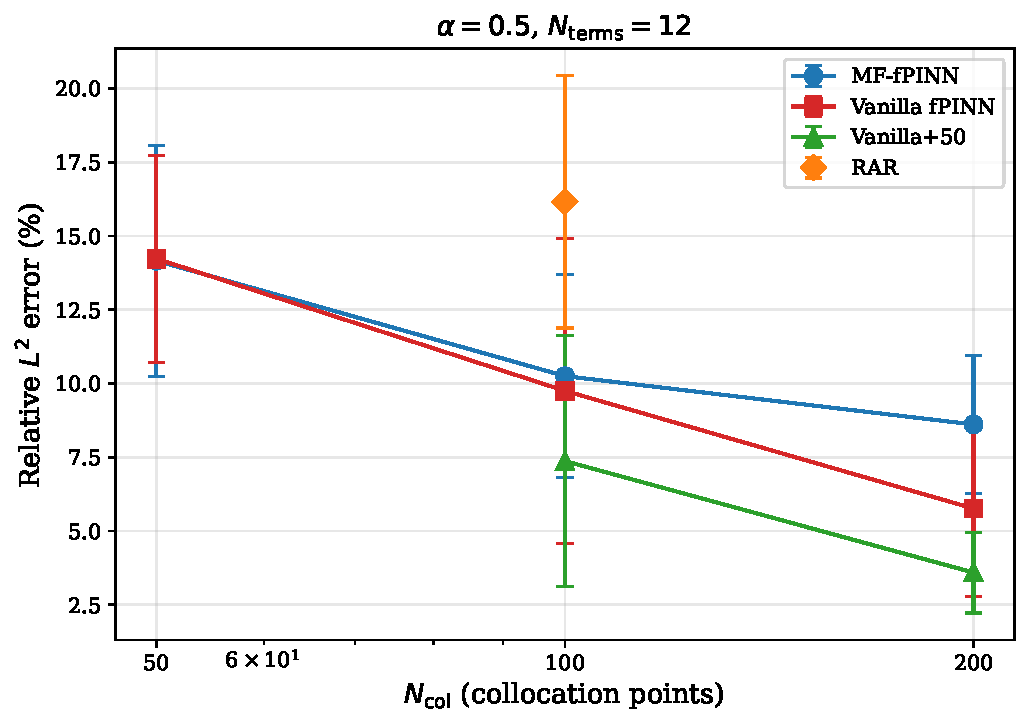
\includegraphics[width=0.65\textwidth]{../figures/ncol_budget_alpha0.5_v2.pdf}
\caption{Collocation budget study at $\alpha = 0.5$ ($N_{\mathrm{terms}} = 12$, 10 seeds). With moderate-quality LF data ($\sim$17\% error), MF-fPINN is comparable to Vanilla at $\Ncol = 100$ ($0.86\times$) and inconsistent at higher budgets. This changes dramatically with higher-quality LF data (see ``Low-fidelity quality controls transfer benefit''). The Vanilla+50 control (adding 50 random collocation points) is the most effective strategy at this LF quality level.}
\label{fig:ncol_budget}
\end{figure}

\subsection{The transfer benefit depends strongly on fractional order}
\label{sec:alpha}

\begin{table}[t]
\centering
\caption{MF-fPINN vs.\ Vanilla across fractional orders at $\Ncol = 100$ ($N_{\mathrm{terms}} = 12$, 10 seeds). MF advantage is strong at $\alpha = 1.0$ ($1.96\times$, $p = 0.010$), absent at $\alpha = 0.5$ ($0.86\times$), and marginal at $\alpha = 0.7$ ($1.18\times$, n.s.).}
\label{tab:alpha_sweep}
\begin{tabular}{rccccc}
\toprule
$\alpha$ & MF (\%) & Vanilla (\%) & Ratio & $p$-value$^\dagger$ & Cohen's $d$ \\
\midrule
0.5 & $6.45 \pm 4.02$ & $5.54 \pm 5.80$ & $0.86\times$ & $0.375$ & $-0.18$ \\
0.7 & $8.44 \pm 7.18$ & $10.00 \pm 8.44$ & $1.18\times$ & $0.432$ & $0.20$ \\
1.0 & $11.81 \pm 6.48$ & $23.15 \pm 13.16$ & $\mathbf{1.96\times}$ & $\mathbf{0.010}$ & $1.09$ \\
\bottomrule
\multicolumn{6}{l}{\small $^\dagger$Two-sided Wilcoxon signed-rank test. Ratio $= $ Vanilla/MF; $>1\times$ favors MF.} \\
\end{tabular}
\end{table}

Table~\ref{tab:alpha_sweep} reveals that MF performance relative to Vanilla varies strongly with $\alpha$. At $\alpha = 0.5$, MF provides no improvement with $N_{\mathrm{terms}} = 12$ LF data ($0.86\times$, $p = 0.375$) because the GL memory provides implicit temporal regularization, making Vanilla already effective ($5.54\%$ at $\Ncol = 100$). At $\alpha = 1.0$, MF achieves a strong and statistically significant advantage ($\mathbf{1.96\times}$, $p = 0.010$, Cohen's $d = 1.09$): without GL memory, the classical PDE provides only one temporal constraint per collocation point, and the MF warm start substantially improves convergence. At $\alpha = 0.7$, MF shows only a marginal, non-significant advantage ($1.18\times$, $p = 0.432$, Cohen's $d = 0.20$), consistent with a smooth transition between the $\alpha = 0.5$ and $\alpha = 1.0$ regimes. The mechanism is clear: classical PDEs ($\alpha = 1$) provide only one temporal constraint per collocation point, while fractional cases ($\alpha < 1$) provide $\mathcal{O}(N_{\mathrm{mem}})$ constraints through the GL sum. Figure~\ref{fig:alpha_advantage} visualizes this trend.

\begin{figure}[t]
\centering
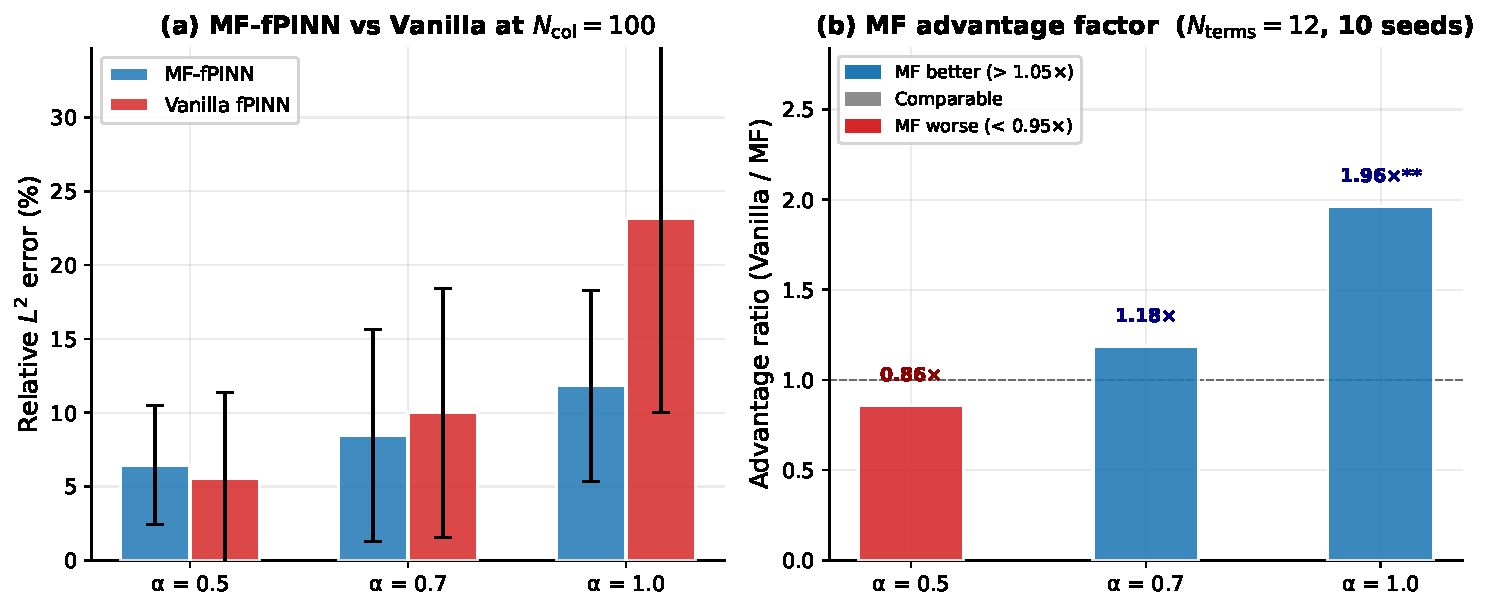
\includegraphics[width=\textwidth]{../figures/alpha_advantage_ncol100.pdf}
\caption{(a) MF-fPINN vs Vanilla fPINN at $\Ncol = 100$ across fractional orders ($N_{\mathrm{terms}} = 12$). (b) Advantage ratio (Vanilla error / MF error); values $>1$ favor MF. At $\alpha = 0.5$, GL memory provides sufficient regularization making MF unnecessary; at $\alpha = 1.0$, MF achieves $1.96\times$ advantage ($p = 0.010$) due to weak PDE signal without GL memory.}
\label{fig:alpha_advantage}
\end{figure}

\subsection{The advantage is not reproduced by adaptive collocation or causal training}
\label{sec:rar}

Residual-adaptive refinement (RAR) \cite{wu2023comprehensive} is the standard approach for improving collocation efficiency without external data. RAR periodically evaluates the PDE residual on a dense candidate set ($n_{\mathrm{cand}} = 5000$ points) and replaces 20\% of collocation points with those having the highest residual, concentrating training on poorly-resolved regions. We perform RAR updates every 2000 epochs.

At $\alpha = 0.5$, $\Ncol = 100$ (5 seeds, $N_{\mathrm{terms}} = 12$, RAR-paired run): RAR achieves $16.16\% \pm 4.79\%$, \emph{worse} than both the paired Vanilla ($9.75\%$) and MF-fPINN ($10.25\%$). One possible explanation consistent with the GL memory mechanism is that since each collocation point already constrains $\sim$100 time steps, the PDE residual is relatively well-distributed even with random collocation; RAR's redistribution may concentrate points in high-residual regions (e.g., the boundary layer) at the expense of interior coverage where GL memory terms are most effective. However, we note that RAR performance is sensitive to implementation details (candidate set size, update frequency, replacement fraction), and our configuration ($n_{\mathrm{cand}} = 5000$, updates every 2000 epochs, 20\% replacement) may not be optimal for this problem. A thorough RAR hyperparameter study is beyond our scope.

Causal training \cite{wang2022respecting} is an alternative approach to improving PINN convergence by imposing temporal causality: the PDE residual at later times is weighted less until earlier-time residuals are satisfied. This addresses a known failure mode where PINNs learn non-causal solutions. If causal training alone matches MF-fPINN, the MF benefit would reduce to ``better training'' rather than genuine data transfer. We implement the causal weighting scheme of \cite{wang2022respecting}: collocation points are sorted into $n_w = 20$ temporal windows, and the PDE residual in window $i$ is weighted by $\exp(-\varepsilon \sum_{j<i} \bar{R}_j)$, where $\bar{R}_j$ is the mean squared residual in window $j$. We sweep $\varepsilon \in \{1, 10, 100\}$, covering gentle to aggressive causal enforcement. Causal training uses the \emph{same} architecture, epoch budget (25{,}000), learning rate ($5 \times 10^{-4}$, cosine decay), collocation budget ($\Ncol = 100$), and random seeds as Vanilla; the only difference is the per-window causal weighting of the PDE loss.

\begin{table}[t]
\centering
\caption{Causal training baseline (Wang et al.\ 2022) vs.\ MF-fPINN and Vanilla (10 seeds, $\Ncol = 100$, $N_{\mathrm{terms}} = 20$ for MF). Causal training is \emph{significantly worse} than Vanilla at both $\alpha$ values across all $\varepsilon$, indicating that the MF advantage stems from data transfer, not improved training dynamics. All $p$-values from two-sided Wilcoxon signed-rank tests vs.\ Vanilla.}
\label{tab:causal}
\begin{tabular}{clccc}
\toprule
$\alpha$ & Method & L2 (\%) & Ratio$^\dagger$ & $p$ (vs.\ Van) \\
\midrule
\multirow{5}{*}{0.5}
& Vanilla           & $5.54 \pm 5.80$  & $1.00\times$ & --- \\
& \textbf{MF-fPINN} & $\mathbf{1.52 \pm 0.75}$  & $\mathbf{3.66\times}$ & $0.002$ \\
& Causal $\varepsilon{=}1$   & $13.21 \pm 5.63$ & $0.42\times$ & $0.004$ \\
& Causal $\varepsilon{=}10$  & $16.22 \pm 5.00$ & $0.34\times$ & $0.002$ \\
& Causal $\varepsilon{=}100$ & $14.30 \pm 7.47$ & $0.39\times$ & $0.002$ \\
\midrule
\multirow{5}{*}{1.0}
& Vanilla           & $23.15 \pm 13.16$ & $1.00\times$ & --- \\
& \textbf{MF-fPINN} & $\mathbf{10.22 \pm 4.56}$  & $\mathbf{2.27\times}$ & $0.006$ \\
& Causal $\varepsilon{=}1$   & $47.62 \pm 8.67$  & $0.49\times$ & $0.004$ \\
& Causal $\varepsilon{=}10$  & $45.82 \pm 8.59$  & $0.51\times$ & $0.004$ \\
& Causal $\varepsilon{=}100$ & $39.20 \pm 22.05$ & $0.59\times$ & $0.010$ \\
\bottomrule
\multicolumn{5}{l}{\small $^\dagger$Ratio = Vanilla error / Method error; values $>1\times$ favor the method.} \\
\end{tabular}
\end{table}

Table~\ref{tab:causal} reveals that causal training is \emph{severely detrimental} for fractional PDEs. At $\alpha = 0.5$, all causal variants are $2.4$--$2.9\times$ worse than Vanilla ($p \leq 0.004$) and $8.7$--$10.7\times$ worse than MF-fPINN ($p = 0.002$). At $\alpha = 1.0$, causal training is $1.7$--$2.1\times$ worse than Vanilla ($p \leq 0.010$). The result is insensitive to $\varepsilon$: all three values produce similar errors, suggesting a fundamental incompatibility rather than a tuning issue.

The likely explanation involves the GL memory structure. At $\alpha = 0.5$, each collocation point's PDE residual depends on $K_{\mathrm{eff}} = 44$ past time steps via the GL weights. The causal weighting scheme, designed for classical ($\alpha = 1$) PDEs where each collocation point depends only on local time, conflicts with this non-local temporal dependence: suppressing contributions from later-time windows also suppresses the GL memory terms that reference those windows from earlier evaluation points. This effectively negates the temporal regularization that makes Vanilla fPINN already effective at $\alpha = 0.5$. At $\alpha = 1.0$ ($K_{\mathrm{eff}} = 2$), the causal scheme should be less antagonistic to GL memory, yet performance is still $\sim$2$\times$ worse---suggesting that at $\Ncol = 100$, the PDE residual is too sparse for window-based reweighting to be effective. This result indicates that the MF advantage cannot be replicated by improved training strategies alone: causal training, the leading PINN training enhancement for temporal PDEs, \emph{hurts} in the fractional setting.

\subsection{Low-fidelity quality controls transfer benefit}
\label{sec:fidelity}

A key question for practitioners is: \emph{how accurate must the LF data be for transfer to help?} We address this from two angles. First, Table~\ref{tab:fidelity_cross} compares MF-fPINN at two LF quality levels across $\alpha$ values at $\Ncol = 100$.

\begin{table}[t]
\centering
\caption{Impact of LF data quality on MF-fPINN across $\alpha$ at $\Ncol = 100$ (10 seeds). With $N_{\mathrm{terms}} = 8$ ($\sim$41\% error at $\alpha = 0.5$, $\sim$25\% at $\alpha = 1.0$), MF \emph{hurts} at both $\alpha$ values ($0.16\times$ and $0.60\times$). With $N_{\mathrm{terms}} = 12$ ($\sim$17\% / $\sim$10\% error), MF is neutral at $\alpha = 0.5$ ($0.86\times$) and significantly beneficial at $\alpha = 1.0$ ($1.80\times$, $p = 0.020$).}
\label{tab:fidelity_cross}
\resizebox{\textwidth}{!}{%
\begin{tabular}{rcccccc}
\toprule
 & \multicolumn{3}{c}{$N_{\mathrm{terms}} = 8$} & \multicolumn{3}{c}{$N_{\mathrm{terms}} = 12$} \\
\cmidrule(lr){2-4} \cmidrule(lr){5-7}
$\alpha$ & MF (\%) & Van (\%) & Ratio & MF (\%) & Van (\%) & Ratio \\
\midrule
0.5 & $34.20 \pm 38.36$ & $5.54 \pm 5.80$ & $0.16\times$ & $6.45 \pm 4.02$ & $5.54 \pm 5.80$ & $0.86\times$ \\
1.0 & $35.30 \pm 22.03$ & $21.28 \pm 13.09$ & $0.60\times$ & $11.80 \pm 6.42$ & $21.28 \pm 13.09$ & $\mathbf{1.80\times}$ \\
\bottomrule
\multicolumn{7}{l}{Ratio = Vanilla error / MF error; $>1\times$ favors MF. All rows: 10 seeds.} \\
\end{tabular}%
}
\end{table}

Table~\ref{tab:fidelity_cross} reveals a striking pattern. At $\alpha = 0.5$, MF is harmful with poor LF data ($N_{\mathrm{terms}} = 8$: $0.16\times$, MF $6\times$ worse) and neutral with moderate data ($N_{\mathrm{terms}} = 12$: $0.86\times$). At $\alpha = 1.0$ with $N_{\mathrm{terms}} = 8$, MF is also harmful ($0.60\times$), but with moderate data ($N_{\mathrm{terms}} = 12$) MF provides a significant benefit ($1.80\times$, $p = 0.020$). This $\alpha$-dependent crossover is consistent with the GL memory mechanism: at $\alpha = 1.0$ without GL memory, the Vanilla baseline is much higher ($21.28\%$ vs.\ $5.54\%$ at $\alpha = 0.5$), leaving more room for the MF warm start to help even with moderate-quality LF data. Figure~\ref{fig:fidelity_cross} visualizes this interaction.

\begin{figure}[t]
\centering
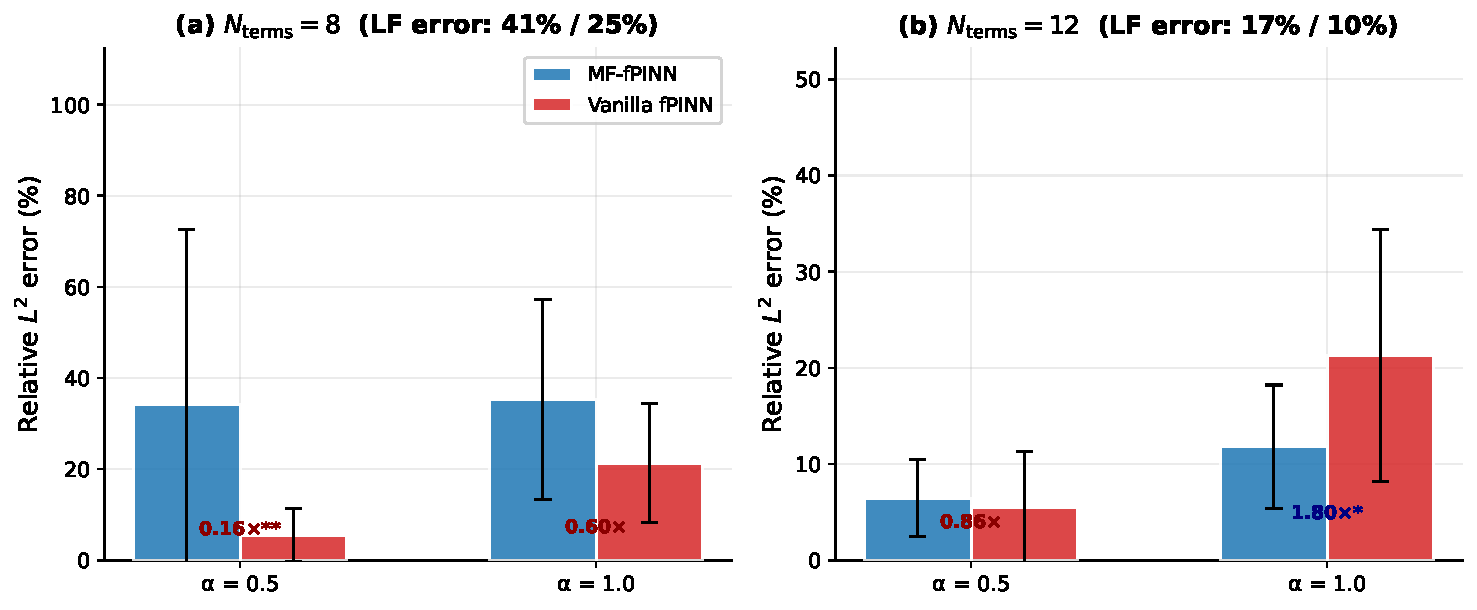
\includegraphics[width=\textwidth]{../figures/fidelity_cross_comparison.pdf}
\caption{Fidelity gap $\times$ $\alpha$ interaction at $\Ncol = 100$ (10 seeds). (a) $N_{\mathrm{terms}} = 8$: MF hurts at both $\alpha$ values ($0.16\times$ at $\alpha = 0.5$, $0.60\times$ at $\alpha = 1.0$). (b) $N_{\mathrm{terms}} = 12$: MF is neutral at $\alpha = 0.5$ ($0.86\times$) but significantly beneficial at $\alpha = 1.0$ ($1.80\times$). The annotated ratios show Vanilla error / MF error ($>1$ favors MF).}
\label{fig:fidelity_cross}
\end{figure}

Second, we systematically vary $N_{\mathrm{terms}} \in \{5, 8, 10, 12, 15, 20\}$ at fixed $\alpha$ and $\Ncol = 100$ to map the transition from detrimental to beneficial transfer. Table~\ref{tab:fidelity_sweep} shows results at $\alpha = 1.0$, where MF transfer is most likely to help.

\begin{table}[t]
\centering
\caption{Fidelity sweep at $\alpha = 1.0$, $\Ncol = 100$ (10 seeds). The advantage ratio increases monotonically beyond $N_{\mathrm{terms}} = 8$: catastrophic at $\sim$71\% LF error ($0.12\times$), crossing unity near $N_{\mathrm{terms}} = 10$ ($1.30\times$, n.s.), and reaching $\mathbf{2.13\times}$ at $N_{\mathrm{terms}} = 20$ ($p = 0.014$). LF errors are relative $L^2$ vs.\ the HF reference on the evaluation grid (same convention as Table~\ref{tab:lf_quality}).}
\label{tab:fidelity_sweep}
\resizebox{\textwidth}{!}{%
\begin{tabular}{rrcccc}
\toprule
$N_{\mathrm{terms}}$ & LF error (\%) & MF (\%) & Van (\%) & Ratio & $p$-value \\
\midrule
5 & 71.2 & $177.48 \pm 156.71$ & & $0.12\times$ & $0.002$ \\
8 & 25.2 & $35.30 \pm 22.03$ & & $0.60\times$ & $0.160$ \\
10 & 15.3 & $16.41 \pm 10.67$ & $21.28 \pm 13.09$ & $1.30\times$ & $0.232$ \\
12 & 10.0 & $11.80 \pm 6.42$ & & $\mathbf{1.80\times}^{*}$ & $\mathbf{0.020}$ \\
15 & 5.5 & $10.72 \pm 4.30$ & & $\mathbf{1.98\times}^{**}$ & $\mathbf{0.010}$ \\
20 & 2.2 & $10.00 \pm 4.59$ & & $\mathbf{2.13\times}^{**}$ & $\mathbf{0.014}$ \\
\bottomrule
\multicolumn{6}{l}{Ratio = Vanilla / MF error; $>1\times$ favors MF. Shared Vanilla baseline, 10 seeds.} \\
\multicolumn{6}{l}{$^{*}$Wilcoxon $p = 0.020$; $^{**}p \leq 0.014$; 95\% bootstrap CI at $N_{\mathrm{terms}} = 20$: $[1.46, 2.84]$.} \\
\end{tabular}%
}
\end{table}

The advantage ratio increases \emph{monotonically} with LF quality at $\alpha = 1.0$, matching the pattern at $\alpha = 0.5$. At $\sim$71\% LF error, the Phase~1 warm start learns a grossly incorrect solution and Phase~2 cannot recover ($0.12\times$). At $\sim$25\% error, MF is still harmful ($0.60\times$, n.s.). The crossover occurs near $N_{\mathrm{terms}} = 10$ ($\sim$15\% LF error, $1.30\times$, $p = 0.232$, n.s.). Beyond this point, the advantage continues to grow: $1.80\times$ at $N_{\mathrm{terms}} = 12$ ($p = 0.020$), $1.98\times$ at $N_{\mathrm{terms}} = 15$ ($p = 0.010$), and $\mathbf{2.13\times}$ at $N_{\mathrm{terms}} = 20$ ($p = 0.014$, 95\% bootstrap CI $[1.46, 2.84]$). Unlike $\alpha = 0.5$, the advantage at $\alpha = 1.0$ appears to saturate near $2\times$, reflecting the reduced variance reduction available without GL memory regularization. Figure~\ref{fig:fidelity_sweep} visualizes this monotonic trend.

\begin{figure}[t]
\centering
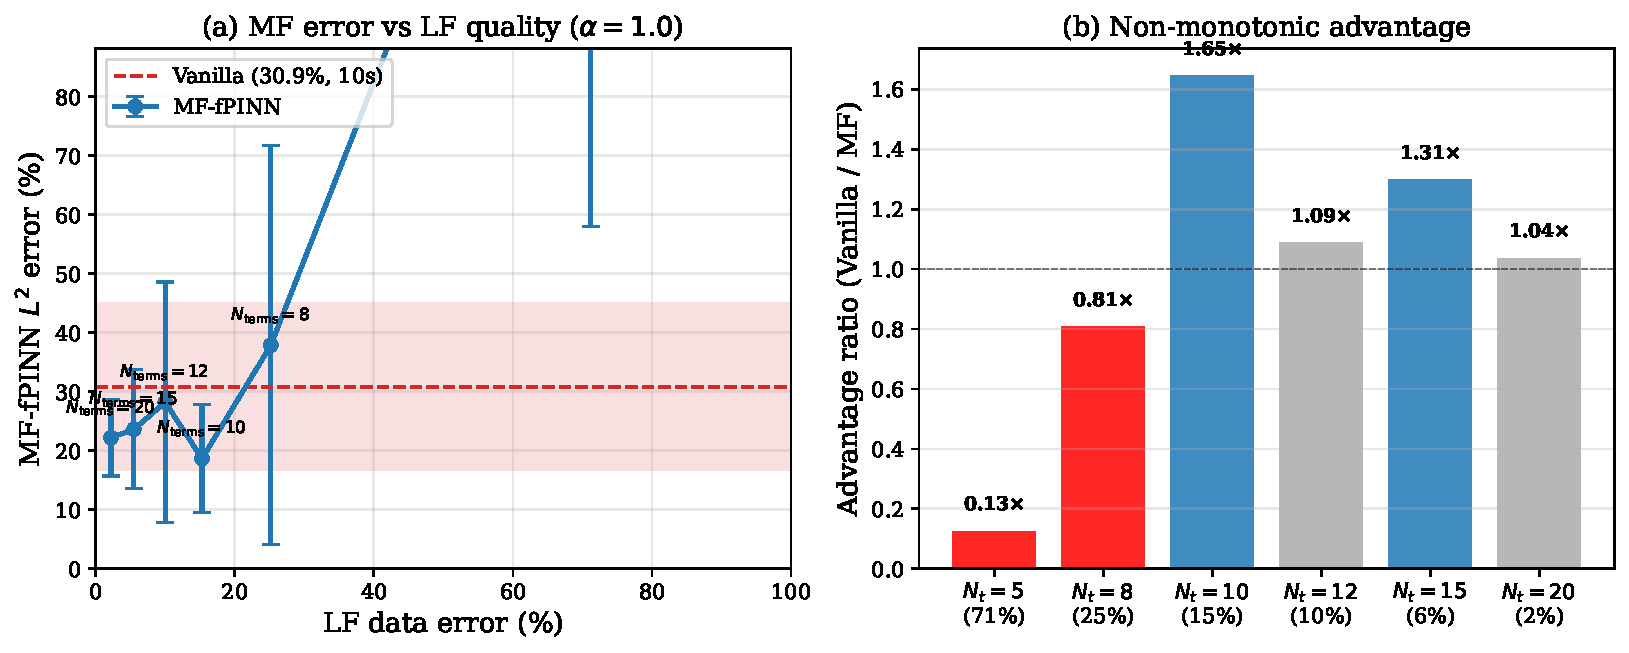
\includegraphics[width=\textwidth]{../figures/fidelity_sweep_alpha1.0.pdf}
\caption{Fidelity sweep at $\alpha = 1.0$, $\Ncol = 100$ (10 seeds). (a) MF-fPINN error as a function of LF data quality (lower $x$-axis = worse LF data). The dashed line and shaded band show Vanilla fPINN $\pm 1\sigma$. (b) Advantage ratio (Vanilla / MF): the advantage increases monotonically, reaching $2.13\times$ at $N_{\mathrm{terms}} = 20$ ($p = 0.014$).}
\label{fig:fidelity_sweep}
\end{figure}

Table~\ref{tab:fidelity_sweep_a05} presents the complementary sweep at $\alpha = 0.5$. Like $\alpha = 1.0$, the advantage ratio is \emph{monotonically increasing} with LF quality: from $0.16\times$ at $N_{\mathrm{terms}} = 8$ (harmful) to $\mathbf{3.66\times}$ at $N_{\mathrm{terms}} = 20$ ($\sim$4\% LF error). This demonstrates that MF transfer \emph{can} provide substantial benefit even at low $\alpha$---but only when the LF data is highly accurate, overcoming the GL memory regularization. At $N_{\mathrm{terms}} = 12$, MF is comparable to Vanilla ($0.86\times$, $p = 0.375$, n.s.), at $N_{\mathrm{terms}} = 15$, MF achieves $2.18\times$ ($p = 0.049$), and at $N_{\mathrm{terms}} = 20$, MF achieves $3.66\times$ ($p = 0.002$, 95\% bootstrap CI $[2.30, 4.83]$)---all with 10 seeds. The approximate crossover from harmful to beneficial occurs near $N_{\mathrm{terms}} \approx 12$ ($\sim$17\% LF error).

\begin{table}[t]
\centering
\caption{Fidelity sweep at $\alpha = 0.5$, $\Ncol = 100$ (10 seeds). Like $\alpha = 1.0$, the advantage increases monotonically with LF quality. MF becomes beneficial only when LF error drops below $\sim$17\%, but reaches $3.66\times$ ($p = 0.002$) with near-HF data ($\sim$4\% error). LF errors are relative $L^2$ vs.\ the HF reference on the evaluation grid (same convention as Table~\ref{tab:lf_quality}).}
\label{tab:fidelity_sweep_a05}
\resizebox{0.9\textwidth}{!}{%
\begin{tabular}{rrcccc}
\toprule
$N_{\mathrm{terms}}$ & LF error (\%) & MF (\%) & Van (\%) & Ratio & $p$-value \\
\midrule
8 & 40.8 & $34.20 \pm 38.36$ & & $0.16\times$ & $0.002$ \\
12 & 16.6 & $6.45 \pm 4.02$ & $5.54 \pm 5.80$ & $0.86\times$ & $0.375$ \\
15 & 9.2 & $2.54 \pm 0.97$ & & $\mathbf{2.18\times}^{*}$ & $\mathbf{0.049}$ \\
20 & 3.7 & $1.52 \pm 0.75$ & & $\mathbf{3.66\times}^{**}$ & $\mathbf{0.002}$ \\
\bottomrule
\multicolumn{6}{l}{Ratio = Vanilla / MF error; $>1\times$ favors MF. Shared Vanilla baseline, 10 seeds.} \\
\multicolumn{6}{l}{$^{*}$Wilcoxon $p = 0.049$, CI $[1.28, 3.19]$. $^{**}p = 0.002$, CI $[2.30, 4.83]$ (10k bootstrap).} \\
\end{tabular}%
}
\end{table}

Both $\alpha$ values display the same monotonic trend, but the \emph{magnitude} differs substantially. At $\alpha = 0.5$, the advantage reaches $3.66\times$ at $N_{\mathrm{terms}} = 20$ ($\sim$4\% LF error), while at $\alpha = 1.0$ it saturates near $2.13\times$ at the same $N_{\mathrm{terms}}$ ($\sim$2\% LF error). The steeper slope at $\alpha = 0.5$ suggests that the MF warm start interacts synergistically with GL memory regularization: when the LF data is sufficiently accurate, Phase~1 provides both a good initialization \emph{and} ongoing data-loss regularization during Phase~2, complementing the GL temporal constraints. At $\alpha = 1.0$, the absence of GL memory limits the achievable variance reduction ($\sim$2$\times$). The practical implication is that for fractional PDEs, investing in LF data quality (e.g., increasing $N_{\mathrm{terms}}$) yields large returns: moving from $N_{\mathrm{terms}} = 12$ to $N_{\mathrm{terms}} = 20$ costs little computationally but improves the advantage from $0.86\times$ to $3.66\times$ ($p = 0.002$) at $\alpha = 0.5$. Figure~\ref{fig:fidelity_sweep_a05} visualizes this monotonic trend.

\begin{figure}[t]
\centering
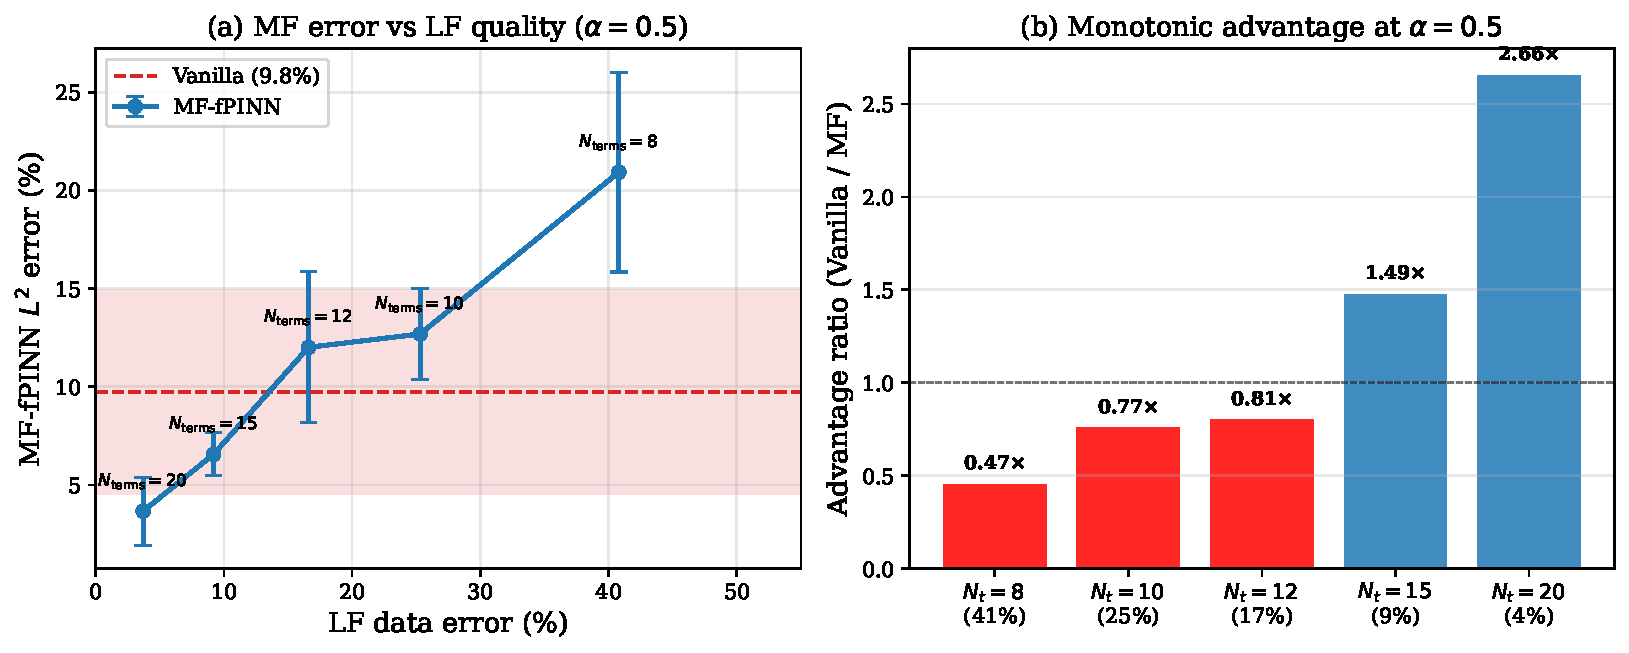
\includegraphics[width=\textwidth]{../figures/fidelity_sweep_alpha0.5.pdf}
\caption{Fidelity sweep at $\alpha = 0.5$, $\Ncol = 100$ (10 seeds). Like $\alpha = 1.0$ (Figure~\ref{fig:fidelity_sweep}), the advantage ratio increases \emph{monotonically} with LF quality: $0.86\times$ at $N_{\mathrm{terms}} = 12$ (n.s.), $2.18\times$ at $N_{\mathrm{terms}} = 15$ ($p = 0.049$), and $3.66\times$ at $N_{\mathrm{terms}} = 20$ ($p = 0.002$). The crossover from harmful to beneficial occurs at $\sim$17\% LF error.}
\label{fig:fidelity_sweep_a05}
\end{figure}

\subsection{Transfer efficiency and noise sensitivity}
\label{sec:transfer}

At $\alpha = 0.5$, $\Ncol = 2000$, $N_{\mathrm{terms}} = 12$, we vary $\NLF \in \{5, 10, 20, 30, 50, 100\}$: MF-fPINN never matches Vanilla (0.66\%), consistent with the GL mechanism---at high $\Ncol$, the PDE loss already provides ample temporal regularization. Varying the data weight $w_{\mathrm{data}} \in \{10, 20, 50\}$ shows insensitivity ($10.25\%$, $9.07\%$, $9.14\%$); LF quality, not weight, is the primary determinant.

We test noise robustness at $\alpha = 1.0$, $\Ncol = 100$ by adding Gaussian noise ($\sigma_\eta \in \{0, 0.01, 0.05, 0.10, 0.20\}$) to the LF data. MF-fPINN is beneficial with clean data ($2.1\times$) and near-clean data ($1.6\times$ at 1\% noise), but degrades rapidly: at 5\% noise, MF already hurts ($0.6\times$), and at 10--20\%, performance deteriorates catastrophically ($0.3\times$ and $0.1\times$). This high sensitivity is consistent with Phase~1's L-BFGS fitting amplifying noise: with only 50 LF points, even 5\% noise substantially corrupts the warm start, and Phase~2's PDE loss at $\alpha = 1.0$ lacks GL memory regularization to correct it. Full results are in Supplementary Section~S4.

\subsection{Grünwald--Letnikov memory changes the value of external data}
\label{sec:gl_ablation}

The preceding experiments establish empirical correlations between $\alpha$, GL memory depth, and MF advantage. To test the \emph{causal} role of GL memory, we conduct a direct ablation: at fixed $\alpha = 0.5$, we artificially truncate the GL memory depth $N_{\mathrm{mem}} \in \{2, 5, 10, 20, 50, 100\}$ and measure both Vanilla and MF-fPINN performance (10 seeds, $\Ncol = 100$, $N_{\mathrm{terms}} = 15$).

The GL memory hypothesis predicts: (i)~Vanilla error should \emph{increase} with truncation (fewer temporal constraints), (ii)~MF error should be \emph{robust} (the warm start compensates), and (iii)~the MF advantage ratio should \emph{increase} with truncation. As a control, we repeat at $\alpha = 1.0$, where $K_{\mathrm{eff}} = 2$ regardless of $N_{\mathrm{mem}}$---truncation should have no effect.

\begin{table}[t]
\centering
\caption{GL memory depth ablation at $\alpha = 0.5$, $\Ncol = 100$, $N_{\mathrm{terms}} = 15$ (10 seeds each). The MF advantage \emph{increases} with GL memory depth: from $1.13\times$ (n.s.) at $N_{\mathrm{mem}} = 2$ to $2.18\times$ ($p = 0.049$) at $N_{\mathrm{mem}} = 100$, as the more accurate fractional derivative provides a stronger PDE loss for Phase~2 refinement. At $\alpha = 1.0$ (control), all $N_{\mathrm{mem}}$ values produce identical results (not shown).}
\label{tab:gl_ablation}
\begin{tabular}{rcccccc}
\toprule
$N_{\mathrm{mem}}$ & Vanilla (\%) & MF-fPINN (\%) & Ratio & $p$-value$^\dagger$ & Cohen's $d$ & Seeds \\
\midrule
  2 & $9.05 \pm 4.23$ & $8.01 \pm 1.12$ & $1.13\times$ & $0.922$ & $0.34$ & 10 \\
  5 & $5.65 \pm 5.01$ & $4.62 \pm 1.09$ & $1.22\times$ & $0.625$ & $0.28$ & 10 \\
 10 & $5.97 \pm 5.26$ & $3.21 \pm 0.98$ & $\mathbf{1.86\times}$ & $\mathbf{0.027}$ & $0.73$ & 10 \\
 20 & $5.44 \pm 5.78$ & $2.69 \pm 0.95$ & $2.03\times$ & $0.064$ & $0.66$ & 10 \\
 50 & $5.36 \pm 5.70$ & $2.51 \pm 0.98$ & $\mathbf{2.14\times}$ & $\mathbf{0.037}$ & $0.70$ & 10 \\
100 & $5.54 \pm 5.80$ & $2.54 \pm 0.97$ & $\mathbf{2.18\times}$ & $\mathbf{0.049}$ & $0.72$ & 10 \\
\bottomrule
\multicolumn{7}{l}{\small $^\dagger$Two-sided Wilcoxon signed-rank test.} \\
\end{tabular}
\end{table}

Table~\ref{tab:gl_ablation} presents the results (all rows 10 seeds). At severe truncation ($N_{\mathrm{mem}} = 2, 5$), both Vanilla and MF performance degrade, and the MF advantage is modest and non-significant ($1.13$--$1.22\times$, $p > 0.6$). With only 2--5 GL terms, the fractional derivative is poorly approximated, and the Phase~2 PDE loss cannot effectively refine the Phase~1 warm start. Interestingly, Vanilla error \emph{increases} under truncation ($9.05\%$ at $N_{\mathrm{mem}} = 2$ vs.\ $5.54\%$ at $N_{\mathrm{mem}} = 100$), confirming that GL terms provide temporal regularization. Beyond $N_{\mathrm{mem}} = 10$, Vanilla performance plateaus at $\sim$5.5\%, while MF continues to improve from $3.21\%$ ($N_{\mathrm{mem}} = 10$) to $2.54\%$ ($N_{\mathrm{mem}} = 100$), driving the advantage from $1.86\times$ to $2.18\times$. At $N_{\mathrm{mem}} = 10, 50, 100$, the advantage is statistically significant ($p < 0.05$), with $N_{\mathrm{mem}} = 20$ marginally non-significant ($p = 0.064$). The $\alpha = 1.0$ experiment produces \emph{identical} Vanilla and MF values across all $N_{\mathrm{mem}}$ (to numerical precision), confirming that the effect is specific to the GL memory structure at $\alpha < 1$. This ablation demonstrates that GL memory depth and MF transfer act \emph{synergistically}: the warm start provides a good initialization that the GL-enriched PDE loss can effectively refine, while Vanilla must navigate the loss landscape from scratch regardless of GL depth.

\subsection{The transfer benefit is time-localized}
\label{sec:time_localization}

The preceding results use the time-averaged relative $L^2$ error $\epsilon_{L^2}$ as the headline metric, which implicitly assumes that the MF advantage is uniformly distributed across the time domain. Resolving the error by individual evaluation time $t \in \{0.05, 0.15, 0.25, 0.40\}$ on a dedicated 10-seed per-timepoint evaluation pool (independently seeded; provenance detailed below) reveals that this assumption fails sharply at $\alpha = 1$, and that the sign of the failure is governed by GL memory.

At $\alpha = 1.0$ with the highest-quality LF data ($N_{\mathrm{terms}} = 20$, ${\sim}2\%$ LF error), MF-fPINN improves the early-time error from $53.7\%$ to $3.9\%$ (a $13.8\times$ reduction), but \emph{degrades} the late-time error from $11.9\%$ to $30.0\%$, an advantage ratio (Vanilla/MF) of $0.40\times$. The per-seed pattern is consistent: MF is better than Vanilla at $t = 0.05$ in $10/10$ seeds and worse at $t = 0.40$ in $8/10$ seeds. This sign reversal is hidden by the time-averaged ratio, which is $2.31\times$ on this independent per-timepoint evaluation pool (the same $\alpha = 1$, $N_{\mathrm{terms}} = 20$ configuration as the headline $2.13\times$ in Table~\ref{tab:fidelity_sweep}, which is computed on the core fidelity-sweep seed pool; the two pools differ as noted in the Experimental setup, Section~\ref{sec:experiments}). Across the full LF sweep at $\alpha = 1.0$, the late-time advantage ratio (Vanilla/MF) saturates near $0.40\times$ regardless of LF quality (ranging from $0.03\times$ at $N_{\mathrm{terms}} = 5$ to $0.40\times$ at $N_{\mathrm{terms}} = 20$): Phase~2 without GL memory cannot prevent late-time drift even when initialized from near-perfect LF data.

At $\alpha = 0.5$ with the same protocol, no such reversal appears. With $N_{\mathrm{terms}} = 20$, all four timepoints show MF better than Vanilla ($5.5\times$, $5.4\times$, $2.4\times$, $2.8\times$ from early to late), with the per-seed late-time inversion occurring in only $2/10$ seeds. The mechanism is consistent with Proposition~\ref{prop:amplification}: the GL sum at $\alpha < 1$ couples the residual at each collocation point to many past time steps, so a Phase~2 gradient step at a late-time point also constrains the network's earlier-time behaviour (and vice versa), allowing the warm start to be refined uniformly across $t$. At $\alpha = 1$ the residual is local in time, so late-time corrections cannot propagate. Figure~\ref{fig:time_localization} visualises both panels.

\begin{figure}[t]
\centering
\includegraphics[width=\textwidth]{../figures/time_localization.pdf}
\caption{Per-timepoint relative $L^2$ error for Vanilla and MF-fPINN at the highest LF quality ($N_{\mathrm{terms}} = 20$, $\Ncol = 100$, 10 seeds; error bars are $\pm 1\sigma$ across seeds). Annotated ratios are Vanilla error / MF error at each timepoint; green indicates MF better, red indicates MF worse. (a)~$\alpha = 0.5$: MF improves all four timepoints ($2.4\times$--$5.5\times$). (b)~$\alpha = 1.0$: MF improves early times by up to $13.8\times$ but \emph{degrades} the late-time error by $2.5\times$ (ratio $0.40\times$), a sign reversal that the time-averaged $2.13\times$ headline conceals.}
\label{fig:time_localization}
\end{figure}

This time-resolved view connects two observations reported elsewhere: the Phase~2 transient degradation at $\alpha = 1$ (Section~\ref{sec:discussion}) is the same late-time error growth observed here, and the apparent $\sim$10\% MF accuracy floor at $\alpha = 1$ is dominated by the late-time component. It also tempers the headline $\alpha = 1$ advantage: the $2.13\times$ time-averaged improvement is a large early-time gain partially offset by a late-time penalty that GL memory does not eliminate because, at $\alpha = 1$, there is no GL memory to eliminate it.

\subsection{Structurally different low-fidelity sources can transfer better}
\label{sec:heterogeneous}

All preceding experiments use degraded Laplace-domain solutions as LF data, which share the same solver structure as the HF reference. A potential concern is that this ``same-solver degradation'' is unrealistically favorable: in practice, LF data often comes from a \emph{structurally different} solver (e.g., coarse finite-difference, reduced-order model). We test whether MF transfer works with data from a qualitatively different LF source. We use an L1 + fully implicit finite-difference (FD) solver on coarse grids: $N_x \in \{3, 5, 10, 20\}$ spatial points with $N_t = 10 N_x$ time steps (the L1 scheme \cite{sun2006fully} approximates the Caputo derivative via backward differences, and fully implicit time-stepping provides unconditional stability; the FD solver is implemented independently from the Laplace solver). This solver introduces \emph{structurally different} errors: spatial discretization truncation and temporal L1 approximation, vs.\ the Laplace solver's spectral truncation in the frequency domain. To ensure a fair comparison, both FD and Laplace LF data are evaluated at the \emph{same} $(\mathbf{x}, t)$ sample locations (via interpolation for FD); only the $u$-values differ.

\begin{table}[t]
\centering
\caption{Heterogeneous LF source: FD solver (L1 scheme) vs.\ Laplace solver as MF-fPINN data source (10 seeds, $\Ncol = 100$, $\NLF = 50$). LF error is measured at the training points vs.\ HF reference. FD LF data matches or \emph{exceeds} Laplace-derived LF at comparable error levels. At $\alpha = 1.0$, FD is $1.3$--$2.0\times$ better than Laplace despite similar or higher LF error, suggesting that structural diversity in the LF source improves transfer.}
\label{tab:heterogeneous}
\begin{tabular}{clcccc}
\toprule
$\alpha$ & LF source & LF err (\%) & L2 (\%) & Ratio$^\dagger$ & $p$ \\
\midrule
\multirow{8}{*}{0.5}
& Vanilla          & ---  & $5.54 \pm 5.80$  & $1.00\times$ & --- \\
& Laplace $N_t{=}20$ & $2.3$ & $1.52 \pm 0.75$  & $3.66\times$ & $0.002$ \\
& Laplace $N_t{=}15$ & $5.6$ & $2.54 \pm 0.97$  & $2.18\times$ & $0.049$ \\
& Laplace $N_t{=}12$ & $9.7$ & $6.45 \pm 4.02$  & $0.86\times$ & $0.375$ \\
\cmidrule{2-6}
& FD $N_x{=}3$  & $3.1$ & $1.57 \pm 0.90$  & $3.52\times$ & $0.004$ \\
& FD $N_x{=}5$  & $2.1$ & $1.47 \pm 0.70$  & $3.78\times$ & $0.004$ \\
& FD $N_x{=}10$ & $1.9$ & $\mathbf{1.33 \pm 0.75}$  & $\mathbf{4.16\times}$ & $0.002$ \\
& FD $N_x{=}20$ & $1.9$ & $1.34 \pm 0.80$  & $4.14\times$ & $0.002$ \\
\midrule
\multirow{8}{*}{1.0}
& Vanilla          & ---  & $23.15 \pm 13.16$ & $1.00\times$ & --- \\
& Laplace $N_t{=}20$ & $1.9$ & $10.22 \pm 4.56$  & $2.27\times$ & $0.006$ \\
& Laplace $N_t{=}15$ & $4.7$ & $10.33 \pm 4.13$  & $2.24\times$ & $0.004$ \\
& Laplace $N_t{=}12$ & $8.4$ & $11.81 \pm 6.48$  & $1.96\times$ & $0.010$ \\
\cmidrule{2-6}
& FD $N_x{=}3$  & $5.9$ & $\mathbf{5.23 \pm 1.14}$   & $\mathbf{4.43\times}$ & $0.002$ \\
& FD $N_x{=}5$  & $2.8$ & $5.82 \pm 1.99$   & $3.98\times$ & $0.002$ \\
& FD $N_x{=}10$ & $1.8$ & $5.89 \pm 3.34$   & $3.93\times$ & $0.004$ \\
& FD $N_x{=}20$ & $1.6$ & $7.58 \pm 4.13$   & $3.05\times$ & $0.004$ \\
\bottomrule
\multicolumn{6}{l}{\small $^\dagger$Ratio = Vanilla error / Method error; values $>1\times$ favor the method.} \\
\end{tabular}
\end{table}

Table~\ref{tab:heterogeneous} presents the results. FD-based LF data consistently matches or \emph{outperforms} Laplace-based LF data. At $\alpha = 0.5$, FD sources achieve $3.52$--$4.16\times$ advantage ($p \leq 0.004$) across all $N_x$ configurations, compared to $3.66\times$ for the best Laplace source. At $\alpha = 1.0$, FD LF data provides \emph{substantially better} transfer than Laplace data at every comparable error level: FD $N_x{=}3$ at $5.9\%$ LF error achieves $4.43\times$ advantage, outperforming even Laplace $N_t{=}20$ at $1.9\%$ error ($2.27\times$). This is striking: the FD source has $3\times$ higher intrinsic error but produces $2\times$ better PINN accuracy. The FD advantage at $\alpha = 1.0$ suggests that \textbf{structural diversity in the LF source may be more important than raw accuracy}: the L1 FD scheme and the Laplace inversion introduce qualitatively different error structures, and these complementary biases may provide a richer initialization in Phase~1 than same-solver degradation. This finding mitigates the ``artificial LF source'' concern by demonstrating that a genuinely different solver produces equal or better transfer. The FD advantage is, however, observed for a single PDE (linear FDR) with smooth solutions and Dirichlet BCs; whether the structural-diversity benefit persists for nonlinear problems, higher-dimensional geometries, or non-smooth solutions remains to be established. The $4.43\times$ figure at $\alpha = 1.0$ should be interpreted as evidence that same-solver degradation is not a best case, rather than as a general claim that coarser solvers are always preferable.

% ================================================================
\section{Discussion}
\label{sec:discussion}
% ================================================================

\textbf{Why study PINNs for this problem.} For the forward problem considered here, the Laplace solver is orders of magnitude faster and more accurate than any PINN, so PINNs are not the method of choice when a fast classical solver is available. The PINN framework becomes valuable in settings where such a solver is unavailable or insufficient: inverse problems in which the boundary forcing, diffusion coefficient, or fractional order $\alpha$ is unknown and must be inferred from data; data-assimilation problems that reconcile sparse, noisy measurements with the governing PDE; and differentiable pipelines that require gradients of the solution with respect to PDE parameters. In these regimes the collocation budget is the dominant training cost, and a warm start that reduces the budget needed to reach a target accuracy is directly useful. Our study therefore treats the well-characterized forward FDR problem as a controlled testbed for \emph{when} multi-fidelity transfer helps fractional PINN training, with the practical payoff residing in the harder settings above; MF-fPINN adds zero wall-time overhead relative to vanilla fPINN (LF data generation costs $<$0.3\,s and the total epoch budget is matched).

\textbf{Why transfer helps at low collocation budget.} The two-phase protocol provides the network with an approximate solution landscape \emph{before} encountering the PDE loss. At low $\Ncol$, the PDE residual may sample the domain too sparsely to provide a useful gradient signal in early training \cite{wang2021understanding}. The Phase~1 warm start can resolve this by providing a rough but global approximation, so Phase~2 only needs to refine local accuracy. However, the strength of this argument depends critically on $\alpha$. At $\alpha = 0.5$, Vanilla fPINN already achieves $\sim$5.5\% error at $\Ncol = 100$ (Table~\ref{tab:ncol}), comparable to MF-fPINN---the GL memory terms provide sufficient temporal coverage even with sparse spatial collocation. The warm start is therefore most impactful at $\alpha = 1.0$, where Vanilla achieves $\sim$23\% error under the same conditions and MF provides a strong $1.96\times$ advantage ($p = 0.010$). At $\alpha = 0.7$, the advantage is marginal ($1.18\times$, $p = 0.432$), confirming the smooth transition between regimes.

\textbf{The learning-rate schedule is not the cause.} A potential confound in the two-phase protocol is that Phase~2 uses a lower learning rate ($\eta = 10^{-4}$, cosine decay over 20{,}000 epochs) than Vanilla ($\eta = 5 \times 10^{-4}$, cosine decay over 25{,}000 epochs). To reduce the likelihood that the MF advantage stems from the LR schedule rather than the data warm start, we run two control experiments. Training Vanilla at $\eta = 10^{-4}$ (matching Phase~2's LR) for 25{,}000 epochs produces \emph{substantially worse} results than the standard $\eta = 5 \times 10^{-4}$ (deposited control \texttt{lr\_control\_results.json}): $12.53\%$ vs.\ $3.62\%$ at $\alpha = 0.5$ ($3.5\times$ worse) and $17.93\%$ vs.\ $5.56\%$ at $\alpha = 0.7$ ($3.2\times$ worse). We also match the MF two-phase \emph{schedule} exactly---5{,}000 epochs at $\eta = 5 \times 10^{-4}$ followed by 20{,}000 epochs at $\eta = 10^{-4}$---but train on PDE loss only (no LF data). This ``vanilla schedule'' isolates the LR schedule effect from the data transfer effect.

The results (Supplementary Table~S9) are unambiguous: the two-phase LR schedule alone is $2.1$--$2.2\times$ \emph{worse} than standard Vanilla across all configurations. MF two-phase outperforms both Vanilla variants by $1.1$--$2.8\times$ vs.\ standard and $2.5$--$5.9\times$ vs.\ the matched schedule. Within the configurations tested, the LR schedule is not the cause of the MF advantage: the observed benefit is attributable to the Phase~1 data warm start, not the learning rate schedule.

\textbf{The fidelity gap threshold.} The fidelity gap threshold depends on both $\alpha$ and the LF quality available. At $\alpha = 0.5$, the crossover from harmful to beneficial MF transfer occurs between $N_{\mathrm{terms}} = 12$ ($\sim$17\% LF error, $0.86\times$) and $N_{\mathrm{terms}} = 15$ ($\sim$9\% LF error, $2.18\times$): below this threshold, MF provides progressively larger gains ($3.66\times$ at $\sim$4\% LF error); above, MF is catastrophically harmful ($0.16\times$ at $\sim$41\% LF error). At $\alpha = 1.0$, the response is \emph{monotonically increasing} with LF quality: advantage grows from $0.12\times$ ($N_{\mathrm{terms}} = 5$, $\sim$71\% error) through $1.30\times$ ($N_{\mathrm{terms}} = 10$, $\sim$15\%) to $2.13\times$ ($N_{\mathrm{terms}} = 20$, $\sim$2\%), with the crossover near $N_{\mathrm{terms}} = 8$ ($\sim$25\%). Both $\alpha$ values exhibit monotonic fidelity responses, but with different crossover thresholds: $\alpha = 0.5$ requires $\lesssim$15\% LF error for benefit, while $\alpha = 1.0$ benefits already at $\lesssim$25\% error. This is consistent with $\alpha = 1.0$'s weaker PDE signal (no GL memory) amplifying the value of \emph{any} reasonable warm start.

\textbf{A bias--variance account.} The fidelity gap threshold can be understood through a bias--variance decomposition, which we refer to below as the bias--variance transfer trade-off (BVTT) framework. For method $M \in \{\text{MF}, \text{Van}\}$ trained with $S$ seeds, $\mathrm{MSE}_M = \mathrm{Bias}^2_M + \mathrm{Var}_M$. MF transfer helps when the variance reduction exceeds the bias increase. Phase~1 constrains the initialization, reducing seed-to-seed variance but introducing systematic LF bias. Computing the decomposition from 10-seed predictions at $\alpha = 0.5$, $\Ncol = 100$ (Supplementary Table~S7) confirms that Vanilla is strongly \emph{variance-dominated} ($87\%$ of MSE). MF's bias scales with LF error: at poor LF quality MF is dominated by LF bias and underperforms, whereas at high LF quality ($N_{\mathrm{terms}} \geq 15$) MF reduces \emph{both} the bias and the prediction standard deviation (the latter by $63$--$79\%$) relative to Vanilla, producing the net advantage. The crossover to net benefit occurs between $N_{\mathrm{terms}} = 12$ and $15$ ($\sim$9--17\% LF error), consistent with the $3.66\times$ advantage at $N_{\mathrm{terms}} = 20$ in Table~\ref{tab:fidelity_sweep_a05}. This decomposition yields a quantitative decision criterion:

\begin{Proposition}[Empirical Scaling Relation (heuristic): crossover threshold for MF benefit]
\label{prop:crossover}
Under the BVTT framework, MF transfer provides net benefit when the LF error $\varepsilon_{\mathrm{LF}}$ satisfies
\begin{equation}
\label{eq:crossover}
\varepsilon_{\mathrm{LF}} < \varepsilon^*(\alpha, \Ncol) = \frac{C}{\sqrt{\Ncol \cdot K_{\mathrm{eff}}(\alpha)}},
\end{equation}
where $C$ depends on the Vanilla variance, variance reduction ratio, and bias sensitivity. Since $K_{\mathrm{eff}}$ decreases with $\alpha$, the threshold $\varepsilon^*$ is most demanding at low $\alpha$.
\end{Proposition}

This is an \emph{empirically calibrated scaling law}, not a general theorem: it assumes the bias--variance structure observed in our FDR experiments ($\mathrm{Bias}^2 \propto \varepsilon_{\mathrm{LF}}^2$, $\mathrm{Var} \propto 1/\Ncol$) and a specific network architecture. The constant $C$ and exponents may shift with different PDE families, network sizes, or training protocols. We present it as a practitioner heuristic that captures the qualitative dependence on $\alpha$ and $\Ncol$, not as a universal bound. Since $K_{\mathrm{eff}}$ decreases with $\alpha$ (Table~\ref{tab:keff}), the formula correctly orders the crossover thresholds: $\varepsilon^*(0.5) < \varepsilon^*(0.7) < \varepsilon^*(1.0)$, meaning the $\alpha = 1.0$ regime tolerates a larger fidelity gap before transfer becomes harmful. This ordering is consistent with the empirical crossovers (${\sim}9$--$17\%$ at $\alpha = 0.5$ versus ${\sim}15$--$25\%$ at $\alpha = 1.0$) in Tables~\ref{tab:fidelity_sweep_a05} and~\ref{tab:fidelity_sweep}. The constant $C \approx 5.8$ is calibrated against the observed crossovers in our data and depends on the Vanilla variance, variance-reduction factor, and bias sensitivity; its precise value should not be used for quantitative extrapolation outside the tested FDR setting.

To assess whether $C \approx 5.8$ depends on the reaction rate $\kappa$, we ran the full fidelity sweep (same protocol: $\Ncol = 100$, $N_{\mathrm{LF}} = 50$, 5 seeds) at $\kappa \in \{0.5, 2.0\}$, bracketing the main value $\kappa = 1.0$. The crossover thresholds are consistent across all three $\kappa$ values. At $\alpha = 0.5$, the crossover from harmful to beneficial MF falls within the $N_{\mathrm{terms}} = 10$--$15$ window ($\sim$9--17\% LF error) for every $\kappa$: between $N_{\mathrm{terms}} = 12$ and $15$ at $\kappa \in \{0.5, 1.0\}$, and between $N_{\mathrm{terms}} = 10$ and $12$ at $\kappa = 2.0$. At $\alpha = 1.0$, the crossover falls between $N_{\mathrm{terms}} = 8$ ($\sim$25\% LF error) and $N_{\mathrm{terms}} = 10$ ($\sim$15\% LF error), also approximately independent of $\kappa$. No individual comparison reaches $p < 0.05$ with 5 seeds (minimum Wilcoxon $p = 0.0625$); the primary evidence is the consistency of the crossover location across $\kappa \in \{0.5, 1.0, 2.0\}$, which supports treating $C$ as approximately reaction-rate-independent within the FDR family studied here.

\textbf{Phase~2 stability.} The BVTT framework predicts that Phase~2 stability depends on $K_{\mathrm{eff}}$. Evaluating L2 error at Phase~2 checkpoints ($N_{\mathrm{terms}} = 20$, $\Ncol = 100$, 5 seeds) confirms this: at $\alpha = 0.5$ ($K_{\mathrm{eff}} = 44$), error decreases monotonically from $114.9\%$ to $3.1\%$; at $\alpha = 1.0$ ($K_{\mathrm{eff}} = 2$), Phase~2 exhibits transient degradation---error drops to $28.9\%$ at 500 epochs, \emph{rises} to $46.2\%$ at 2{,}000, then slowly recovers to $22.2\%$ at 20{,}000. This transient is the same late-time error growth quantified in Section~\ref{sec:time_localization}: the $46.2\%$ peak is dominated by the $t = 0.40$ component, and the partial recovery to $22.2\%$ leaves the residual $0.40\times$ advantage ratio (Vanilla/MF) at late time documented there. Both are manifestations of Phase~2's inability to propagate corrections backward in time at $\alpha = 1$, where the GL sum reduces to two adjacent time-step weights. At $\alpha \approx 1$, early stopping or a reduced Phase~2 learning rate therefore mitigates the visible symptom but not the underlying limitation. A more targeted remedy suggested by the time-resolved analysis is a temporally weighted Phase~2 PDE loss---for example, weighting collocation residuals by a descending function of $t$, or by $1/K_{\mathrm{eff}}(\alpha, t)$ in a depth-aware variant---to suppress late-time drift without altering the GL discretization itself; we have not implemented or tested this, and leave it for future work. A GL-aware adaptive schedule ($\eta \propto \sqrt{K_{\mathrm{eff}}/2}$, $E \propto 1/\sqrt{K_{\mathrm{eff}}/2}$) reduces Phase~2 compute by $2$--$3\times$ at low $\alpha$ with minimal accuracy loss at $\alpha \geq 0.9$. Full results are in Supplementary Section~S6.

\textbf{GL memory as implicit temporal regularization.} The GL discretization evaluates the model at $K_{\mathrm{eff}}(\alpha)$ past time steps per collocation point (Proposition~\ref{prop:amplification}): $K_{\mathrm{eff}} = 44$ at $\alpha = 0.5$ versus 2 at $\alpha = 1$. While temporally correlated, this $5$--$22\times$ increase in evaluations is consistent with Vanilla achieving $\sim$5.5\% error at $\alpha = 0.5$ but $\sim$23\% at $\alpha = 1.0$ under identical settings (Table~\ref{tab:ncol}). This qualifies, for the FDR equation studied here, the common assumption that fractional PDEs are uniformly ``harder'' for PINNs: while per-point GL computation is more expensive, the memory terms provide a richer gradient signal during training (Figure~\ref{fig:gl_memory}). The direct ablation (``Grünwald--Letnikov memory changes the value of external data'') provides the strongest evidence: as GL depth increases, MF advantage grows ($1.13\times$ at $N_{\mathrm{mem}} = 2$ to $2.18\times$ at $N_{\mathrm{mem}} = 100$), Vanilla error increases under truncation, and the $\alpha = 1.0$ control (identical results across all $N_{\mathrm{mem}}$) rules out confounds. The time-resolved analysis in Section~\ref{sec:time_localization} sharpens this picture: at $\alpha < 1$ the GL sum lets a single Phase~2 gradient step couple the residual at one collocation point to many earlier time steps, so late-time corrections propagate backward and the warm start is refined uniformly across $t$; at $\alpha = 1$ the residual is local in time and late-time error cannot be eliminated, regardless of LF quality. This constitutes a controlled intervention rather than an observational correlation, though we cannot exclude that loss landscape topology or gradient flow patterns also contribute. For the specific 1D problem studied, the Laplace solver is orders of magnitude faster ($\sim$90\,s for a dense HF grid vs.\ $\sim$580\,s per PINN run at lower accuracy); the PINN framework is justified for amortized inference, inverse problems, or integration into differentiable pipelines, and \emph{within} the PINN framework, MF-fPINN adds zero wall-time overhead (LF data generation $<$0.3\,s; total epochs match Vanilla).

\begin{figure}[t]
\centering
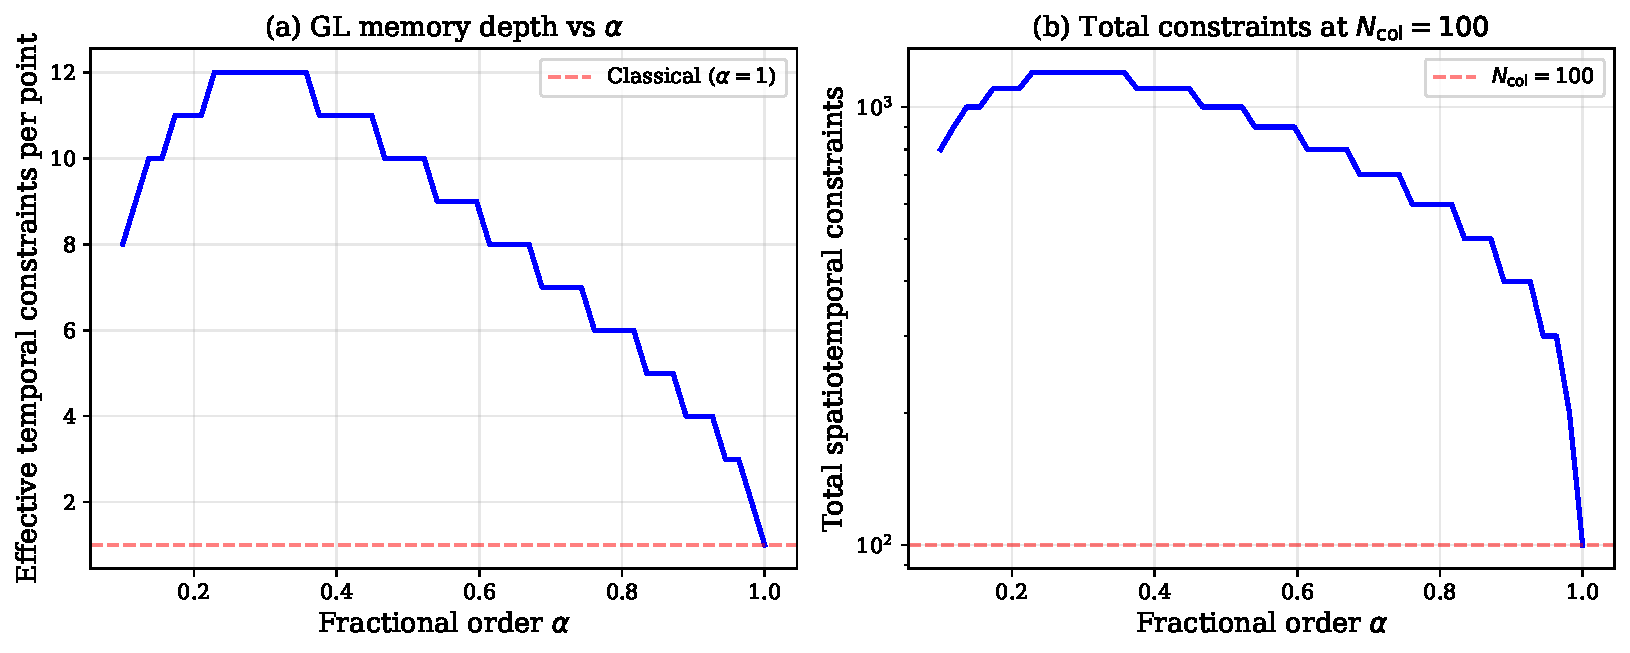
\includegraphics[width=\textwidth]{../figures/gl_memory_mechanism.pdf}
\caption{GL memory mechanism. (a) Number of non-negligible GL weights as a function of $\alpha$, consistent with $K_{\mathrm{eff}}$ in Table~\ref{tab:keff}. (b) Total effective spatiotemporal constraints at $\Ncol = 100$.}
\label{fig:gl_memory}
\end{figure}

\textbf{Practitioner guidelines.} Based on our experiments, we offer the following empirical decision rules for applying multi-fidelity transfer to fractional PINNs. (1)~\emph{Invest in LF quality above all}: LF data quality is the single most important factor; at $\alpha = 0.5$, improving from $N_{\mathrm{terms}} = 12$ to $20$ is computationally cheap but transforms the MF advantage from $0.86\times$ to $3.66\times$, and Scaling Relation~\ref{prop:crossover} can be used to predict benefit. (2)~\emph{MF transfer benefits low collocation budgets most}: the advantage concentrates at low $\Ncol$ ($\leq 200$) and narrows with increasing budget, though at $\alpha = 1.0$ it persists across budget levels ($1.96$--$2.11\times$). (3)~\emph{At low $\alpha$ with moderate LF data, add collocation instead}: the Vanilla+50 control outperforms MF transfer when GL memory already provides rich temporal regularization and LF quality is only moderate ($\gtrsim$15\% error). (4)~\emph{Consider structurally diverse LF sources}: at $\alpha = 1.0$, an L1 FD solver at $5.9\%$ LF error achieves $4.43\times$ advantage, outperforming a Laplace source at $1.9\%$ error ($2.27\times$). (5)~\emph{At $\alpha \approx 1$, consider Phase~2 early stopping}, since Phase~2 exhibits transient degradation at $\alpha = 1.0$.

\textbf{Limitations.} Supplementary Table~S10 summarises the four multi-PDE and higher-dimensional stress-test outcomes from Supplementary Sections~S1--S3 (the noise-robustness stress test is reported separately in Supplementary Section~S4). We note the following limitations.
\begin{enumerate}
\item \emph{Dependence on a usable LF source.} MF-fPINN requires an LF solver that is both cheap enough to justify the two-phase overhead and accurate enough to cross the fidelity threshold ($\lesssim$15\% error at $\alpha = 0.5$, $\lesssim$25\% at $\alpha = 1.0$). The heterogeneous LF experiment partially mitigates the ``artificial LF'' concern, but was demonstrated on a single linear PDE.
\item \emph{Hard BC requirement.} 2D experiments with soft BCs yield $0.47$--$0.65\times$ even with near-perfect LF data---a structural requirement limiting applicability to problems where hard BC ansatze can be constructed.
\item \emph{Mechanism partially isolated.} The GL ablation provides a controlled intervention with an $\alpha = 1.0$ null control. However, Vanilla performance saturates beyond $N_{\mathrm{mem}} \approx 10$, and we cannot rule out that loss landscape topology also contributes.
\item \emph{Low-dimensional scope.} Experiments cover 1D and 2D spatial domains; extension to 3D and coupled systems requires addressing GL memory cost and more complex BC structures.
\item \emph{Statistical power.} Most configurations use 5 seeds (minimum two-sided Wilcoxon $p = 0.062$); key comparisons use 10 seeds. Under Holm--Bonferroni step-down correction at family-wise $\alpha_{\mathrm{fw}} = 0.05$, the two pre-specified primary hypotheses ($\alpha = 0.5$ fidelity at $N_{\mathrm{terms}} = 20$, $p = 0.002$; $\alpha = 1.0$ fidelity at $N_{\mathrm{terms}} = 20$, $p = 0.014$) both survive, and all remaining comparisons are treated as exploratory.
\item \emph{The $\alpha=1$ advantage is early-time-concentrated.} The time-resolved analysis (Section~\ref{sec:time_localization}) shows that at $\alpha = 1$ the $2.13\times$ time-averaged improvement is a $13.8\times$ early-time gain partially offset by a $0.40\times$ late-time penalty that persists across all LF qualities. The headline ratio is correct, but should be interpreted with this structural decomposition in mind.
\item \emph{PINN-internal comparison.} For this benchmark, classical numerical methods are cheaper and more accurate, so our comparisons are between PINN-internal strategies.
\item \emph{Resolved confounds.} The LR schedule control rules out the inter-phase LR difference, and the gradient clipping discrepancy (1.0 vs.\ 5.0) \emph{favors Vanilla}, making reported MF advantages conservative.
\end{enumerate}

\textbf{Summary.} The practical contribution is a decision rule: across the full fractional range tested, MF transfer becomes beneficial once the LF error falls below a memory-dependent threshold ($\lesssim$15\% at $\alpha = 0.5$, $\lesssim$25\% at $\alpha = 1$), yielding up to a $3.66\times$ reduction in relative $L^2$ error, and is counterproductive above it. Using degraded Laplace-domain solutions as tunable low-fidelity data, we mapped the interaction between collocation budget, fidelity gap, and fractional order, with stress tests on nonlinear and higher-dimensional PDEs. LF data quality is the dominant factor: at $\alpha = 0.5$, improving LF quality from $\sim$17\% error to $\sim$4\% transforms MF-fPINN from neutral ($0.86\times$) to strongly beneficial ($3.66\times$, $p = 0.002$, survives Holm--Bonferroni), while at $\alpha = 1.0$ the response increases monotonically to $2.13\times$ at $\sim$2\% error ($p = 0.014$). We formalized GL memory's implicit regularization (Propositions~\ref{prop:keff}--\ref{prop:amplification}) and tested it with a controlled ablation whose direction matches the prediction, with an $\alpha = 1.0$ null control. Stress tests delineate the method's boundary of applicability: nonlinear Burgers at $\alpha = 1$ yields $2.25\times$ but at $\alpha < 1$ the singular Caputo correction makes MF counterproductive; soft BC enforcement in 2D is associated with consistent failure; and a parametric $\alpha$-PINN inverts the per-$\alpha$ findings. Structurally different LF data (L1 finite-difference) can outperform same-solver degradation, while causal training is severely incompatible with fractional residuals. The practical implication, restricted to the settings tested, is that MF-fPINN provides substantial benefit when LF quality is high ($\lesssim$5\% error) at any tested $\alpha$, or when LF quality is moderate ($\sim$15--25\% error) and GL memory is weak ($\alpha \gtrsim 0.7$). For strongly fractional PDEs ($\alpha \lesssim 0.5$) with only moderate LF quality, additional collocation appears more cost-effective than MF transfer. Future work includes extension to 3D coupled systems, improved parametric $\alpha$-PINN training, and integration of GL-aware adaptive schedules into reproducible workflows.

% ================================================================
\section{Methods}
\label{sec:methods}
% ================================================================

\subsection{Fractional diffusion--reaction equation}
\label{sec:problem}

Consider the time-fractional diffusion-reaction equation on $\Omega = (0, L) \times (0, T]$:
\begin{equation}
\label{eq:fdr}
\partial_t^\alpha u = D \frac{\partial^2 u}{\partial x^2} - \kappa u, \quad x \in (0, L),\; t > 0,
\end{equation}
with boundary conditions \cite{podlubny1999fractional}
\begin{equation}
u(0, t) = g(t), \quad u(L, t) = 0,
\end{equation}
and initial condition $u(x, 0) = 0$, where $\partial_t^\alpha$ denotes the Caputo fractional derivative of order $\alpha \in (0, 1]$:
\begin{equation}
\label{eq:caputo}
\partial_t^\alpha u(x,t) = \frac{1}{\Gamma(1-\alpha)} \int_0^t \frac{\partial u(x,\tau)}{\partial \tau} (t - \tau)^{-\alpha} \diff\tau.
\end{equation}
The physical parameters are diffusion coefficient $D > 0$ and reaction rate $\kappa \geq 0$. We use $g(t) = \sin(\pi t / a)$ for $t \in [0, a]$ and $g(t) = 0$ otherwise, with $a = 0.5$. The function $g$ is continuous on $[0, T]$ but not differentiable at $t = a$; this regularity is consistent with the Caputo formulation in~\eqref{eq:caputo} and is reflected in the inversion-error structure reported below.

\subsection{Laplace-domain solution}
\label{sec:laplace}

Applying the Laplace transform $\bar{u}(x,s) = \int_0^\infty u(x,t) e^{-st}\diff t$ and using $u(x,0) = 0$ (so Caputo = Riemann--Liouville), Eq.~\eqref{eq:fdr} becomes the ODE
\begin{equation}
D\, \bar{u}_{xx} - (s^\alpha + \kappa)\, \bar{u} = 0,
\end{equation}
with solution
\begin{equation}
\label{eq:laplace_solution}
\bar{u}(x, s) = \bar{g}(s) \cdot \frac{\sinh\bigl(\lambda(L-x)\bigr)}{\sinh(\lambda L)}, \quad \lambda = \sqrt{\frac{s^\alpha + \kappa}{D}}.
\end{equation}
The time-domain solution is recovered via numerical inverse Laplace transform using the Valsa--Brancik algorithm \cite{valsa2001approximate} with $N_{\mathrm{terms}}$ terms at $p$-digit precision using the \texttt{mpmath} library.

\subsection{Multi-fidelity data generation}
\label{sec:mf_data}

A key design choice is how LF data is generated. Rather than using a different solver or surrogate, we degrade the \emph{same} Laplace-domain solver by reducing $N_{\mathrm{terms}}$ (number of Laplace inversion terms) and arithmetic precision. The high-fidelity (HF) configuration uses $N_{\mathrm{terms}} = 30$ and precision $= 30$ decimal digits; the low-fidelity (LF) configuration uses $N_{\mathrm{terms}} \in \{5, 8, 10, 12, 15, 20\}$ and precision $= 20$ decimal digits. This produces a controllable fidelity gap: at $\alpha = 0.5$, LF error ranges from $\sim$124\% ($N_{\mathrm{terms}} = 5$, essentially useless) to $\sim$4\% ($N_{\mathrm{terms}} = 20$, nearly HF quality). This laboratory-like control over the fidelity gap enables systematic study of the fidelity--performance relationship without confounding factors from heterogeneous solvers; real multi-fidelity scenarios may exhibit qualitatively different bias structures, and the quantitative thresholds derived here should be treated as problem-specific. Table~\ref{tab:lf_quality} shows the LF error as a function of $N_{\mathrm{terms}}$ and $\alpha$. Crucially, LF error increases with decreasing $\alpha$---the Laplace inversion for fractional-order problems is more sensitive to truncation. At $\alpha = 1.0$, the same $N_{\mathrm{terms}} = 12$ gives only 10\% error vs.\ 17\% at $\alpha = 0.5$. Our default LF configuration uses $N_{\mathrm{terms}} = 12$ and $\NLF = 50$ LF training points at random $(x, t)$ locations.

\begin{table}[t]
\centering
\caption{LF data quality (relative $L^2$ error vs.\ HF, \%) as a function of Laplace inversion terms $N_{\mathrm{terms}}$ and fractional order $\alpha$. Precision fixed at 20 digits. Lower $\alpha$ produces higher LF error due to increased sensitivity of the Laplace inversion to term count.}
\label{tab:lf_quality}
\begin{tabular}{rccccc}
\toprule
$N_{\mathrm{terms}}$ & $\alpha = 0.3$ & $\alpha = 0.5$ & $\alpha = 0.7$ & $\alpha = 0.9$ & $\alpha = 1.0$ \\
\midrule
5 & 130.9 & 123.7 & 111.8 & 96.2 & 71.2 \\
8 & 51.2 & 40.8 & 40.5 & 33.2 & 25.2 \\
10 & 32.9 & 25.3 & 25.2 & 20.2 & 15.3 \\
12 & 21.7 & 16.6 & 16.1 & 12.7 & 10.0 \\
15 & 12.4 & 9.2 & 8.9 & 7.0 & 5.5 \\
20 & 5.1 & 3.7 & 3.5 & 2.7 & 2.2 \\
\bottomrule
\end{tabular}
\end{table}

\subsection{Network architecture}

We use a fully-connected neural network $\hat{u}_\theta(x, t)$ with random Fourier features \cite{tancik2020fourier,wang2021eigenvector} as input encoding:
\begin{equation}
\gamma(x, t) = \left[\cos(2\pi \bm{B} [x, t]^\top),\; \sin(2\pi \bm{B} [x, t]^\top)\right], \quad B_{ij} \sim \mathcal{N}(0, \sigma^2),
\end{equation}
where $\sigma$ controls the frequency bandwidth. The encoded features pass through $N_L$ hidden layers with $N_H$ neurons each and $\tanh$ activation. Boundary and initial conditions are enforced exactly via the ansatz
\begin{equation}
\label{eq:hard_bc}
\hat{u}(x, t) = g(t)\frac{L-x}{L} + x(L-x)\,t\,\mathrm{NN}_\theta(x, t),
\end{equation}
which guarantees $\hat{u}(0,t) = g(t)$, $\hat{u}(L,t) = 0$, and $\hat{u}(x,0) = 0$ (since $g(0) = 0$). This eliminates BC/IC losses entirely, leaving only the PDE residual and optional data loss.

\subsection{Loss functions}

For $\alpha < 1$, the Caputo derivative is approximated via the Gr\"unwald--Letnikov (GL) scheme \cite{meerschaert2004finite,podlubny1999fractional,diethelm2002numerical}:
\begin{equation}
\label{eq:gl}
\partial_t^\alpha u(x, t) \approx h^{-\alpha} \sum_{k=0}^{N_{\mathrm{mem}}} w_k\, u(x, t - kh),
\end{equation}
where $h$ is the time step, $w_0 = 1$, $w_k = w_{k-1}(1 - (1+\alpha)/k)$, and $N_{\mathrm{mem}} = \min(\lfloor t_{\max}/h \rfloor, N_{\mathrm{max}})$ is bounded by a maximum memory depth $N_{\mathrm{max}}$. We use $h = 0.01$ and $N_{\mathrm{max}} = 100$, so the GL sum evaluates the network at up to 100 past time steps per collocation point. The memory length is computed from $t_{\max}$ (the maximum time in the collocation batch) rather than per-point $t_i$ to enable batched evaluation. For collocation points where $t_i - kh < 0$, the shifted time is clamped to $0$; since the initial condition enforces $\hat{u}(x, 0) = 0$ via the hard BC ansatz, this is equivalent to zero-extension and introduces no additional approximation error. Since $u(x,0) = 0$ holds exactly, the GL and Caputo operators coincide for this problem \cite{podlubny1999fractional}, validating the use of GL weights for the Caputo residual throughout. For $\alpha = 1$, we bypass the GL scheme and use standard autograd $\partial u / \partial t$. The PDE loss is
\begin{equation}
\Lcal_{\mathrm{PDE}} = \frac{1}{\Ncol} \sum_{i=1}^{\Ncol} \left[\partial_t^\alpha \hat{u}(x_i, t_i) - D\, \hat{u}_{xx}(x_i, t_i) + \kappa\, \hat{u}(x_i, t_i)\right]^2.
\end{equation}
Given LF data $\{(x_j^{\mathrm{LF}}, t_j^{\mathrm{LF}}, u_j^{\mathrm{LF}})\}_{j=1}^{\NLF}$, the data loss is
\begin{equation}
\Lcal_{\mathrm{data}} = \frac{1}{\NLF} \sum_{j=1}^{\NLF} \left[\hat{u}(x_j^{\mathrm{LF}}, t_j^{\mathrm{LF}}) - u_j^{\mathrm{LF}}\right]^2.
\end{equation}
Collocation points $(x_i, t_i)$ are sampled from a Beta-biased distribution $x \sim \mathrm{Beta}(0.5, 2.0)$, $t \sim 0.01 + (T - 0.01) \cdot \mathrm{Beta}(0.5, 2.0)$, which concentrates points near the left boundary and early times where the solution has the steepest gradients. Points are resampled every 1000 epochs to improve coverage over training.

\subsection{Two-phase training protocol}
\label{sec:twophase}

\begin{algorithm}[h]
\caption{MF-fPINN Two-Phase Training}
\label{alg:mf}
\begin{algorithmic}[1]
\REQUIRE LF data $\mathcal{D}_{\mathrm{LF}}$, collocation budget $\Ncol$, physics parameters
\STATE \textbf{Phase 1} (Data pre-training, $E_1$ epochs):
\STATE \quad Minimize $\Lcal_{\mathrm{data}}$ with Adam ($\mathrm{lr} = 5 \times 10^{-4}$, cosine annealing)
\STATE \quad L-BFGS polish (50 steps) to tightly fit the $\NLF$ LF data points
\STATE \textbf{Phase 2} (Physics-informed fine-tuning, $E_2$ epochs):
\STATE \quad \textbf{Fresh} Adam optimizer ($\mathrm{lr} = 10^{-4}$, cosine annealing)
\STATE \quad Minimize $w_{\mathrm{PDE}}(e) \cdot \Lcal_{\mathrm{PDE}} + w_{\mathrm{data}} \cdot \Lcal_{\mathrm{data}}$
\STATE \quad where $w_{\mathrm{PDE}}(e) = \min(1, e/E_{\mathrm{ramp}})$ ramps up PDE weight ($E_{\mathrm{ramp}} = 3{,}000$)
\RETURN Trained model $\hat{u}_\theta$
\end{algorithmic}
\end{algorithm}

Phase~1 provides a warm start by fitting the network to sparse LF data, concluding with L-BFGS refinement to achieve tight data fitting (a trivial 50-point regression costing $<$1 second). Phase~2 uses a \emph{fresh} optimizer (resetting Adam momentum) and gradually ramps up the PDE weight over $E_{\mathrm{ramp}}$ epochs to avoid destabilizing the pre-trained weights. The data loss is retained in Phase~2 as regularization with weight $w_{\mathrm{data}} = 10$. Phase~1 evaluates the model on 50 points ($\mathcal{O}(\NLF)$ per epoch), while Phase~2 evaluates the GL fractional derivative on $\Ncol$ points ($\mathcal{O}(\Ncol \cdot N_{\mathrm{mem}})$ per epoch). For our default $\Ncol = 100$ and $N_{\mathrm{mem}} = 100$, Phase~1 is $\sim$200$\times$ cheaper per epoch than Phase~2. The total wall time for MF-fPINN training is $E_1 + E_2$ epochs, equal to the Vanilla baseline. Empirically, at $\alpha = 0.5$, $\Ncol = 100$: MF-fPINN $\approx 582$s, Vanilla $\approx 590$s, RAR $\approx 580$s per run on a single NVIDIA GPU. The vanilla fPINN trains for $E_1 + E_2$ epochs on $\Lcal_{\mathrm{PDE}}$ only, ensuring equal total training budget. The RAR baseline \cite{wu2023comprehensive} periodically evaluates the PDE residual on a dense candidate set ($n_{\mathrm{cand}} = 5000$) and replaces 20\% of collocation points with those having the highest residual every 2000 epochs.

\subsection{GL memory as implicit regularization: analysis}
\label{sec:gl_theory}

We now formalize the observation that the GL discretization~\eqref{eq:gl} provides implicit temporal regularization whose strength depends on $\alpha$.

\begin{Proposition}[GL weight asymptotics and effective constraint count]
\label{prop:keff}
Let $\{w_k\}_{k=0}^{N_{\mathrm{mem}}}$ be the GL weights defined by $w_0 = 1$, $w_k = w_{k-1}(1-(1+\alpha)/k)$. Then:
\begin{enumerate}
\item[(i)] For $\alpha = 1$: $w_0 = 1$, $w_1 = -1$, and $w_k = 0$ for all $k \geq 2$.
\item[(ii)] For $\alpha \in (0,1)$: $|w_k| \sim k^{-(1+\alpha)} / |\Gamma(-\alpha)|$ as $k \to \infty$.
\item[(iii)] Define the effective temporal constraint count at threshold $\varepsilon > 0$ as
\begin{equation}
\label{eq:keff}
K_{\mathrm{eff}}(\alpha, \varepsilon) = \bigl|\{k \in \{0, \ldots, N_{\mathrm{mem}}\} : |w_k| > \varepsilon\}\bigr|.
\end{equation}
Then $K_{\mathrm{eff}}(1, \varepsilon) = 2$ for all $\varepsilon < 1$, while for $\alpha \in (0,1)$,
\begin{equation}
K_{\mathrm{eff}}(\alpha, \varepsilon) \leq \min\bigl(N_{\mathrm{mem}}+1,\; C\,(\varepsilon\,|\Gamma(-\alpha)|)^{-1/(1+\alpha)}\bigr),
\end{equation}
for an absolute constant $C \geq 1$ absorbing the asymptotic remainder in~(ii). The bound is non-increasing in $\alpha$ for $\alpha$ near $1$, and observed to decrease monotonically on the grid $\{0.3, 0.5, 0.7, 0.9, 1.0\}$ (Table~\ref{tab:keff}).
\end{enumerate}
\end{Proposition}

\begin{proof}
(i) Direct computation: $w_1 = 1 \cdot (1 - 2/1) = -1$ and $w_2 = -1 \cdot (1 - 2/2) = 0$, with the recurrence preserving $w_k = 0$ for $k \geq 2$.
(ii) The GL weights are $w_k = (-1)^k \binom{\alpha}{k}$, where $\binom{\alpha}{k} = \alpha(\alpha-1)\cdots(\alpha-k+1)/k!$. By the asymptotic expansion of the generalized binomial coefficient \cite{podlubny1999fractional,li2015numerical}, $|\binom{\alpha}{k}| \sim k^{-(1+\alpha)}/|\Gamma(-\alpha)|$ as $k \to \infty$ for $\alpha \notin \mathbb{N}$, giving $|w_k| \sim k^{-(1+\alpha)}/|\Gamma(-\alpha)|$.
(iii) From (ii), $|w_k| > \varepsilon$ requires $k \lesssim (\varepsilon\,|\Gamma(-\alpha)|)^{-1/(1+\alpha)}$, giving the stated bound. As $\alpha \to 1^-$, $|\Gamma(-\alpha)| \to \infty$ (pole of $\Gamma$ at $-1$), so the upper bound $(\varepsilon|\Gamma(-\alpha)|)^{-1/(1+\alpha)} \to 0$, consistent with limiting case~(i). Note that $|\Gamma(-\alpha)|$ is not globally monotone on $(0,1)$ (it has poles at both $\alpha \to 0^+$ and $\alpha \to 1^-$), so the bound alone does not establish monotonicity of $K_{\mathrm{eff}}$ across the full interval; the non-increasing behaviour in Table~\ref{tab:keff} over $\{0.3,0.5,0.7,0.9,1.0\}$ is an empirical observation from the computed weights.
\end{proof}

\begin{table}[t]
\centering
\caption{Effective temporal constraint count $K_{\mathrm{eff}}(\alpha, \varepsilon)$ from the GL weights ($N_{\mathrm{mem}} = 100$, $h = 0.01$). At $\alpha = 1$, only 2 weights are nonzero (finite difference). At $\alpha = 0.3$, 66 weights exceed the $\varepsilon = 10^{-3}$ threshold, providing $33\times$ more temporal constraints per collocation point.}
\label{tab:keff}
\begin{tabular}{rccccc}
\toprule
$\alpha$ & 0.3 & 0.5 & 0.7 & 0.9 & 1.0 \\
\midrule
$K_{\mathrm{eff}}(\alpha, 10^{-2})$ & 12 & 10 & 7 & 4 & 2 \\
$K_{\mathrm{eff}}(\alpha, 10^{-3})$ & 66 & 44 & 26 & 12 & 2 \\
\bottomrule
\end{tabular}
\end{table}

\begin{Proposition}[Effective temporal evaluation count]
\label{prop:amplification}
Consider the PDE loss $\Lcal_{\mathrm{PDE}} = \Ncol^{-1} \sum_{i=1}^{\Ncol} \Rcal_i^2$, where the residual at each collocation point is
\[
\Rcal_i = h^{-\alpha} \sum_{k=0}^{N_{\mathrm{mem}}} w_k\, \hat{u}_\theta(x_i, t_i - kh) - D\,\hat{u}_{xx}(x_i, t_i) + \kappa\,\hat{u}(x_i, t_i).
\]
The gradient $\partial \Lcal_{\mathrm{PDE}} / \partial \theta$ involves the network Jacobian $\partial \hat{u}_\theta / \partial \theta$ evaluated at up to $K_{\mathrm{eff}}(\alpha, \varepsilon)$ distinct temporal locations per collocation point. Define the \emph{temporal evaluation ratio}
\begin{equation}
\label{eq:lambda}
\Lambda(\alpha) = \frac{K_{\mathrm{eff}}(\alpha, \varepsilon)}{K_{\mathrm{eff}}(1, \varepsilon)} = \frac{K_{\mathrm{eff}}(\alpha, \varepsilon)}{2}.
\end{equation}
Then $\Ncol$ collocation points at fractional order $\alpha$ produce gradient contributions from $\Ncol \cdot K_{\mathrm{eff}}(\alpha, \varepsilon)$ distinct spatiotemporal evaluations, vs.\ only $2\Ncol$ at $\alpha = 1$. \textbf{Important caveat:} these additional evaluations share the same spatial location $x_i$ (they are temporally correlated along a single spatial trajectory), so their information content is \emph{not} equivalent to $K_{\mathrm{eff}}$ independent spatiotemporal collocation points. Nevertheless, they constrain the network's temporal behavior at each spatial location, providing implicit temporal regularization absent in the classical case. At $\varepsilon = 10^{-3}$: $\Lambda(0.3) \approx 33$, $\Lambda(0.5) \approx 22$, $\Lambda(0.7) \approx 13$, $\Lambda(0.9) \approx 6$.
\end{Proposition}

\begin{proof}
Expanding $\partial \Rcal_i / \partial \theta$ via the chain rule:
\[
\frac{\partial \Rcal_i}{\partial \theta} = h^{-\alpha} \sum_{k=0}^{N_{\mathrm{mem}}} w_k \frac{\partial \hat{u}_\theta}{\partial \theta}\bigl(x_i, t_i - kh\bigr) + \text{(spatial terms at }(x_i, t_i)\text{)}.
\]
The first sum couples the gradient to the Jacobian at $K_{\mathrm{eff}}$ distinct temporal locations (those with $|w_k| > \varepsilon$). For $\alpha = 1$, this reduces to $(1/h)[\partial \hat{u}_\theta/\partial\theta(x_i,t_i) - \partial \hat{u}_\theta/\partial\theta(x_i,t_i-h)]$, involving only 2 temporal locations. The ratio $\Lambda$ thus measures how many more temporal evaluations per collocation point are generated by the fractional derivative relative to the classical case.
\end{proof}

We additionally probed whether GL memory improves conditioning at initialization in the neural tangent kernel (NTK) framework \cite{wang2022ntk}. Computing the full Jacobian $J_{ij} = \partial \Rcal_i/\partial\theta_j$ and the NTK matrix $K = JJ^\top$ for a small network (3 layers, 32 neurons, 3201 parameters) at 30 collocation points across 5 random seeds yields a \emph{null finding}: the condition number $\kappa(K)$ varies by only $\sim$5\% across $\alpha$ ($5.67 \times 10^5$ at $\alpha = 0.3$ vs.\ $5.41 \times 10^5$ at $\alpha = 1.0$), the effective rank is essentially unchanged ($\approx 6.6$), and $\lambda_{\max}$/$\lambda_{\min}$ shows no meaningful $\alpha$-dependence. This null finding extends to the production network (5 layers, 128 neurons, 82{,}689 parameters; same 30 collocation points and 5 random seeds): $\kappa(K)$ varies by only $\sim$8\% across $\alpha$ ($7.82 \times 10^5$ at $\alpha = 0.3$ vs.\ $7.23 \times 10^5$ at $\alpha = 1.0$), the effective rank again $\approx 6.3$. GL memory therefore does not improve NTK conditioning at initialization regardless of network size; any benefit appears to manifest \emph{during training} through the gradient structure of Proposition~\ref{prop:amplification}.

\subsection{Hardware and software}

All experiments were run on NVIDIA RTX A6000 GPUs (48\,GB VRAM, driver 535.288.01). The software stack is: Python 3.10.12, PyTorch 2.7.1 (CUDA 11.8), mpmath 1.3.0 (arbitrary-precision Laplace inversion), NumPy 2.1.3, and SciPy 1.15.3. Effect sizes are reported as Cohen's $d$ using the pooled standard deviation (Bessel-corrected, $\mathrm{ddof} = 1$); because the design is paired (same random seed), we treat $d$ as a descriptive magnitude only, with all inference based on the paired Wilcoxon signed-rank tests. For key advantage ratios, we additionally report 95\% bootstrap confidence intervals (10{,}000 resamples).

% ================================================================
\section*{Data availability}
% ================================================================
The full reproducibility package, including the seed-level JSON files underlying every table and figure (core fidelity, collocation, $\alpha$-sweep, GL-memory ablation, per-timepoint, bias--variance, and all stress-test, control, and ablation experiments), together with a table-to-source map, is openly available at \url{https://github.com/ammarlhassan/fractional-pinn-transfer}. A small number of inline diagnostic sweeps (the Phase-2 stability checkpoint curves in Supplementary Section~S6 and the $\NLF$/data-weight transfer-efficiency sweeps reported in the Results) are not stored as standalone JSON but are reproduced directly by the deposited experiment scripts (e.g.\ \texttt{run\_phase2\_stability.py}, \texttt{run\_fdr\_anneal\_sweep.py}).

\section*{Code availability}
The code implementing the MF-fPINN two-phase protocol, the Laplace and L1 finite-difference solvers, and all experiment scripts is openly available at \url{https://github.com/ammarlhassan/fractional-pinn-transfer}.

\section*{Author contributions}
A.T., Y.R.\ and A.A.E.L.\ conceived the study. A.T.\ developed the methodology and software, and conducted the formal analysis, investigation, data curation, and visualization. A.T., Y.R.\ and S.A.\ performed validation. A.T.\ wrote the original draft; A.T., Y.R., S.A.\ and A.A.E.L.\ reviewed and edited the manuscript. Y.R.\ and A.A.E.L.\ supervised the work. All authors read and approved the final manuscript.

\section*{Competing interests}
The authors declare no competing interests.

\section*{Acknowledgements}
The authors thank Alamein International University (AIU) for computational resources. This research received no external funding.

%% ---- References -------------------------------------------------------
\bibliographystyle{unsrt}
\bibliography{references}

\end{document}
